\documentclass[fyp]{socreport}
\usepackage{fullpage}
\usepackage{parskip}
\usepackage{graphicx}
\usepackage{tabularx}
\usepackage[table,xcdraw]{xcolor}
\graphicspath{ {img/} }
\begin{document}
\pagenumbering{roman}
\title{NUSWorks: A Student Workload Tool}
\author{Wang Zhipeng}
\projyear{2016/17}
\projnumber{H098960}
\advisor{Dr. Bimlesh Wadhwa}
\deliverables{
	\item Report: 1 Volume}
\maketitle
\begin{abstract}
Student workload is a important factor that may decide whether a student could have a good balance between life and study. The aim of this project is to model the student workload for National University of Singapore (NUS) undergraduates. Meanwhile, develop a student workload prediction tool for NUS undergraduates using machine learning algorithm based on these models. As for doing this, I will review the research papers related to student workload in higher education, build the student workload models to quantify workload of NUS undergraduates, and develop the workload prediction tool application based on the workload models. Also, this paper will discuss the architecture and technologies of the application.

\begin{descriptors}
	\item D.2.2 Design Tools and Techniques
  \item I.2.6 Learning (K.3.2)
	\item K.3 Computers and Education
\end{descriptors}
\begin{keywords}
	Student workload, workload model, web application, software engineering, machine learning
\end{keywords}
\begin{implement}
	React, React-Redux, Material-UI, Python 3.6, Flask, MariaDB
\end{implement}
\end{abstract}

\begin{acknowledgement}
First of all, I would like thank Dr. Bimlesh Wadhwa for her unconditional support and mentorship, and helping me review research papers and giving suggestions for report and prototype implementation. Also, I like to thank my teammate Tran Cong Thien for our good cooperation and helpful suggestions about this project. Last but not least, I would like to thank my family and my friends for their continuous and sincere support.
\end{acknowledgement}

% \listoffigures
% \listoftables
\tableofcontents

\chapter{Introduction}

\section{Background}
\subsection{Workload is important for both teaching staff and students}
Nowadays, student workload has become one of the important factors in the higher education, and it is also an important condition for student to have a good balance between study and life (Kember, 2004). In addition, one study from Kyle Bowyer shows that around one third of students from Organization for Economic Co-operation and Development (OECD) countries drop their studies before finishing, and student workload, as a study-related factor, plays an important role for causing the dropout (Bowyer, 2012). Thus, studying for student workload should be beneficial for both students to have an appropriate workload and higher education institutes to arrange reasonable workload for each course.

\subsection{Workload is hard to measure}
It may be difficult to measure the student workload as some number. Studies show that student workload is simply measured as number of studying hours per week (Kember, 2004), but some researchers have indicated that student workload is hard to estimate because student workload may not only related to worked time per week, but also be influenced by other factors like teaching method for each course and personal capability of each student (Ruiz-Gallardo, Castaño, Gómez- Alday \& Valdés, 2009). Meanwhile, student workload can be classified into two parts where one is objective workload that is measured by time, and the other is subjective workload which can be defined as the effect of factors related to student, such as effort and confusion (Kyndt, Berghmans, Dochy \& Bulckens, 2014). Therefore, student workload is not easily estimated by time and calculation of student workload may require plenty of factors which may be hard to find and measure.

\subsection{No such tool in NUS for undergraduate}
Since student workload is important for student in education aspect, some universities have developed workload tools either for their students or for teaching staff to manage student workload or course workload. Nonetheless, there is still no such tool for NUS undergraduates to maintain their study workload. Thus, there is a need of student workload tool for NUS undergraduates which may help them manage their workload in a reasonable and easy-understanding manner.

\subsection{Machine learning in predicting education workload}
In addition, machine learning, as known as a subset of artificial intelligence, has been used  in many aspects such as education. For example, use machine learning to analyse and track student learning and provide recommendation for future learning, and build a grade system using machine learning to evaluate and assess student performance (Ark, 2015). However, current there is no such a tool using machine learning to manage student workload, and it could be helpful if we can use machine learning technology to manage student workload.

\section{Motivation}
Since currently there is no such tool for NUS undergraduates, it could be helpful if I design and develop a workload tool to assist undergraduate students in managing their workload. In addition, as an NUS Computer Science undergraduate, I would appreciate an opportunity to facilitate NUS undergraduate student learning process.

\section{Objective}
\subsection{Help student understand their workload by prediction}
Most importantly, NUSWorks mainly aims to develop a workload prediction web application to help NUS undergraduates understand and manage their workload by predicting their possible workload within one semester, and visualising the resulting workload in an interactive and user- friendly way.

\subsection{More accurate measure of workload if more info provided}
Besides, NUSWorks can accept varied amount of input information and use different models to predict. If users (i.e. NUS undergraduates) provide more information, the result of predicted workload will be more accurate.

\subsection{Use machine learning to improve prediction accuracy}
Meanwhile, machine learning is a powerful technology that it can modify the models based on more training data provided and it could be more accurate after training. Thus, NUSWorks aims to increase the accuracy by applying machine learning technology.

\section{Scope}
\subsection{Prediction of workload}
Several models will be built to describe student workload. The models should be reasonable and well-tested and the results should be easily understood by students.

\subsection{Visualisation of workload}
The prediction results of models should be presented in a way that user can understand it easily and can manipulate some data through the user interface in a user-friendly way.

\subsection{Accessibility of tool}
Allow user to log in with his or her NUS Integrated Virtual Learning Environment (IVLE) account. Also, they can choose to use the workload tool without logging in.

\subsection{Model refinement}
Integrate machine learning methods so that the prediction models might become more accurate if more workload data can be collected and analysed to improve the model.

\subsection{Model variety}
Allow user to choose either enter partial information or full information, and different models will be applied based on the input.

\chapter{Literature Review}
% \label{ch:related}
\section{Workload Understanding}
\subsection{General definition of workload}
Generally, workload has become one of the most significant factor that will affect the quality of teaching and learning (Giles, 2007; Kyndt, Dochy, Struyven \& Cascallar, 2011a). Moreover, based on studies on workload, researchers prefer to have two different categories of workload where one is objective workload, and the other is subjective workload, also known as perceived workload (Kyndt et al., 2014).

\subsection{Objective workload}
Usually, objective workload refers to the number of study hours that students spend (Kyndt et al., 2014). Although sometimes objective workload is one efficient way to represent the student workload and it is easy to measure, it is not enough. For example, two modules may have the same number of working hours per week, but students may think one has heavier workload than the other. Thus, it is usually insufficient that people only use objective workload to measure the whole student workload.

\subsection{Subjective workload}
Subjective workload is introduced to supplement objective workload. It consists of requirements for students and the consequences resulted from these requirements (Kyndt et al., 2014). However, due to the subjective nature of this concept, it is difficult to be measured accurately. For example, learning environment can be considered as one factor influencing subjective workload, but it is hard to measure it since it cannot be represented by a number.

\section{Workload Assessment}
\subsection{General approaches}
Different approaches have been used to assess student workload by other researchers. Some researchers use open questions to collect student feedback for workload through survey (Kingsland, 1996; Lizzio, Wilson, \& Simons, 2002; Reisslein, Tylavsky, Matar, Seeling, \& Reisslein., 2007; Solomon \& Finch, 1998), but students may be influenced by their perceived difficulty or relationship between teachers and students (Ruiz-Gallardo et al., 2009).

Besides, students are usually asked to fill some evaluation form at the end of semester, and there may be some questions asking the amount of time student has spent per week (Greenwald \& Gillmore, 1997; Lawless, 2000; Zuriff, 2003). However, the problem is that it may be hard for student to recall weekly working time (Chambers, 1992). Meanwhile, students may also be affected by subjective factors of courses (Garg, Vijayshre, \& Panda, 1992).

Lastly, based on the estimation of time students spend on different assessments, one approach is to calculate the time and teacher can adjust the syllabus before course starts (Chambers, 1992; Chambers, 1994). On the one hand, the advantages of this method is that it does not require student actions, and it is helpful for teachers to plan their courses appropriately before starting. On the other hand, the estimated result may not be accurate.

\subsection{Existing workload model}
A student workload model proposed by Bowyer (2012) has been reviewed. The model is created after finding all possible factors that may influence student workload, and making those factors quantified. In his paper, he summarises that there are 4 different categories of factors which are difficulty, time, ability, and effort. He tries to quantifying the factors based on a set of experiments. Table \ref{factor-table} shows how the factors are quantified.

\begin{table}[]
\centering
\begin{tabular}{|p{0.15\textwidth}|p{0.85\textwidth}|}
\hline
\rowcolor[HTML]{E0E0E0}
\textbf{Difficulty} & \textbf{(InherentDifficulty + AssessmentDifficulty) / 2} \newline InherentDifficulty=((AttributeDifficulty / NumberOfAttributes) * Year / 18) * (1 - DisciplineDifficulty) \newline AssessmentDifficulty=(AssessmentPreparation + Duration) / Marks * Memorises * Modules / (Week + WeekSince) \\
\hline
\textbf{Time} & The least time one student have to spend to pass a course is the preparation time, attending university assessments time, and individual study time. \\
\hline
\rowcolor[HTML]{E0E0E0}
\textbf{Ability} & This mainly consists of two parts: student academic ability and experienced credits. For freshie undergraduates, can use average (i.e. 50) for its student academic ability. \\
\hline
\textbf{Effort} & This is included because it is very important for student to put in effort in common sense. Here he uses time needed to pass at average effort and time needed to pass at full effort as a measure of effort (former one should more the later one). \\
\hline
\end{tabular}
\caption{Quantification of Workload Factors}
\label{factor-table}
\end{table}

For these four factors, he indicates that they are helpful for university teachers to make a appropriate teaching plan. For difficulty, teachers can adjust the syllabus and lower is difficulty of assessments. For time, teachers can see if there is reasonable amount of time for individual learning, and if the time needed to pass is too high. For Ability, teachers can suggest whether it is appropriate for a student to take this course with certain ability. Lastly, for effort, teachers can adjust the syllabus if too much or too little effort needed to pass.

\section{Existing Workload Tool}
There are several existing workload tools either for students or teachers.

\subsection{An existing workload tool from Rice University}
The first one is from Rice University which is a workload tool for student. It is a web application that student can use it to calculate weekly working hours based on the reading and writing assignments, exams and other assignments.

For reading assignment, student can enter factors including pages per week, page density, difficulty and purpose. Besides, student can adjust the reading rate manually which by default is 67 pages per hour. For writing assignment, student can enter factors including pages per semester, page density, genre and drafting, and student also can adjust the writing rate which by default is 0.75 hours per page. Figure {\ref{rice-1}} is a screenshot of the workload tool.

\begin{figure}
\frame{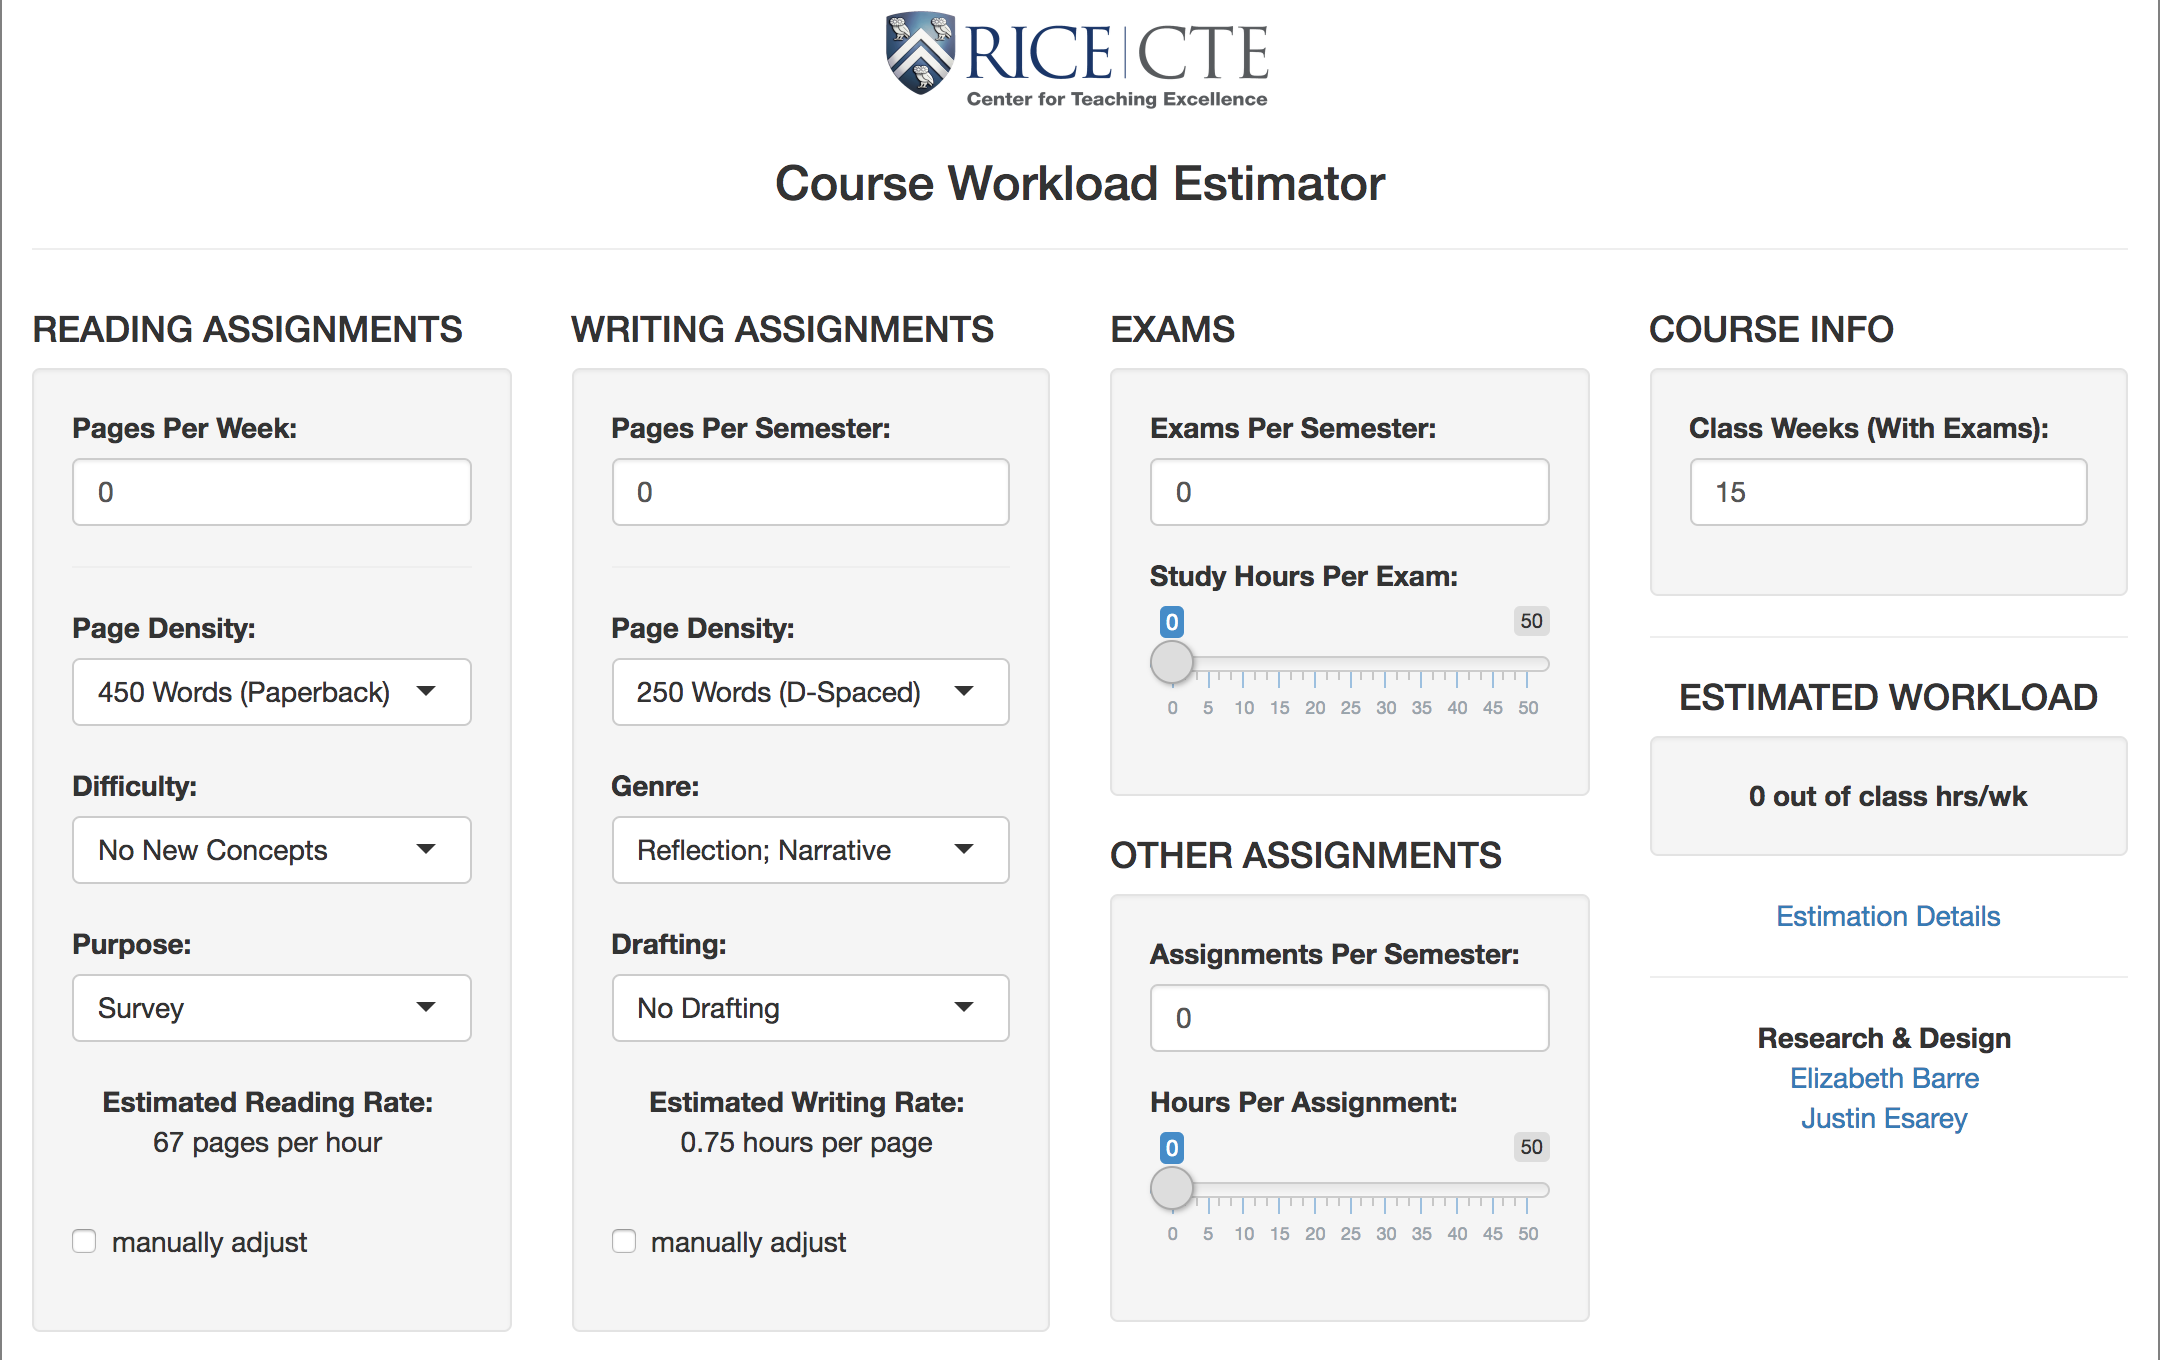
\includegraphics[width=\textwidth]{rice-university}}
\caption{Rice University Course Workload Estimator}
\label{rice-1}
\end{figure}

\subsection{An existing workload tool from Massey University}
This tool, in fact, is for students who study remotely instead of staying at school. Firstly, student will choose the number of papers he or she would like to take for coming semester. Then student will enters how many hours he or she plans to spend on several categories of activities per week, such as sleeping, working and exercising. After those two steps, the tool will calculate the total number of hours the student will spend. Figure {\ref{massey-1}} is a screenshot of this tool and Figure {\ref{massey-2}} shows the calculated result of workload.

\begin{figure}
\frame{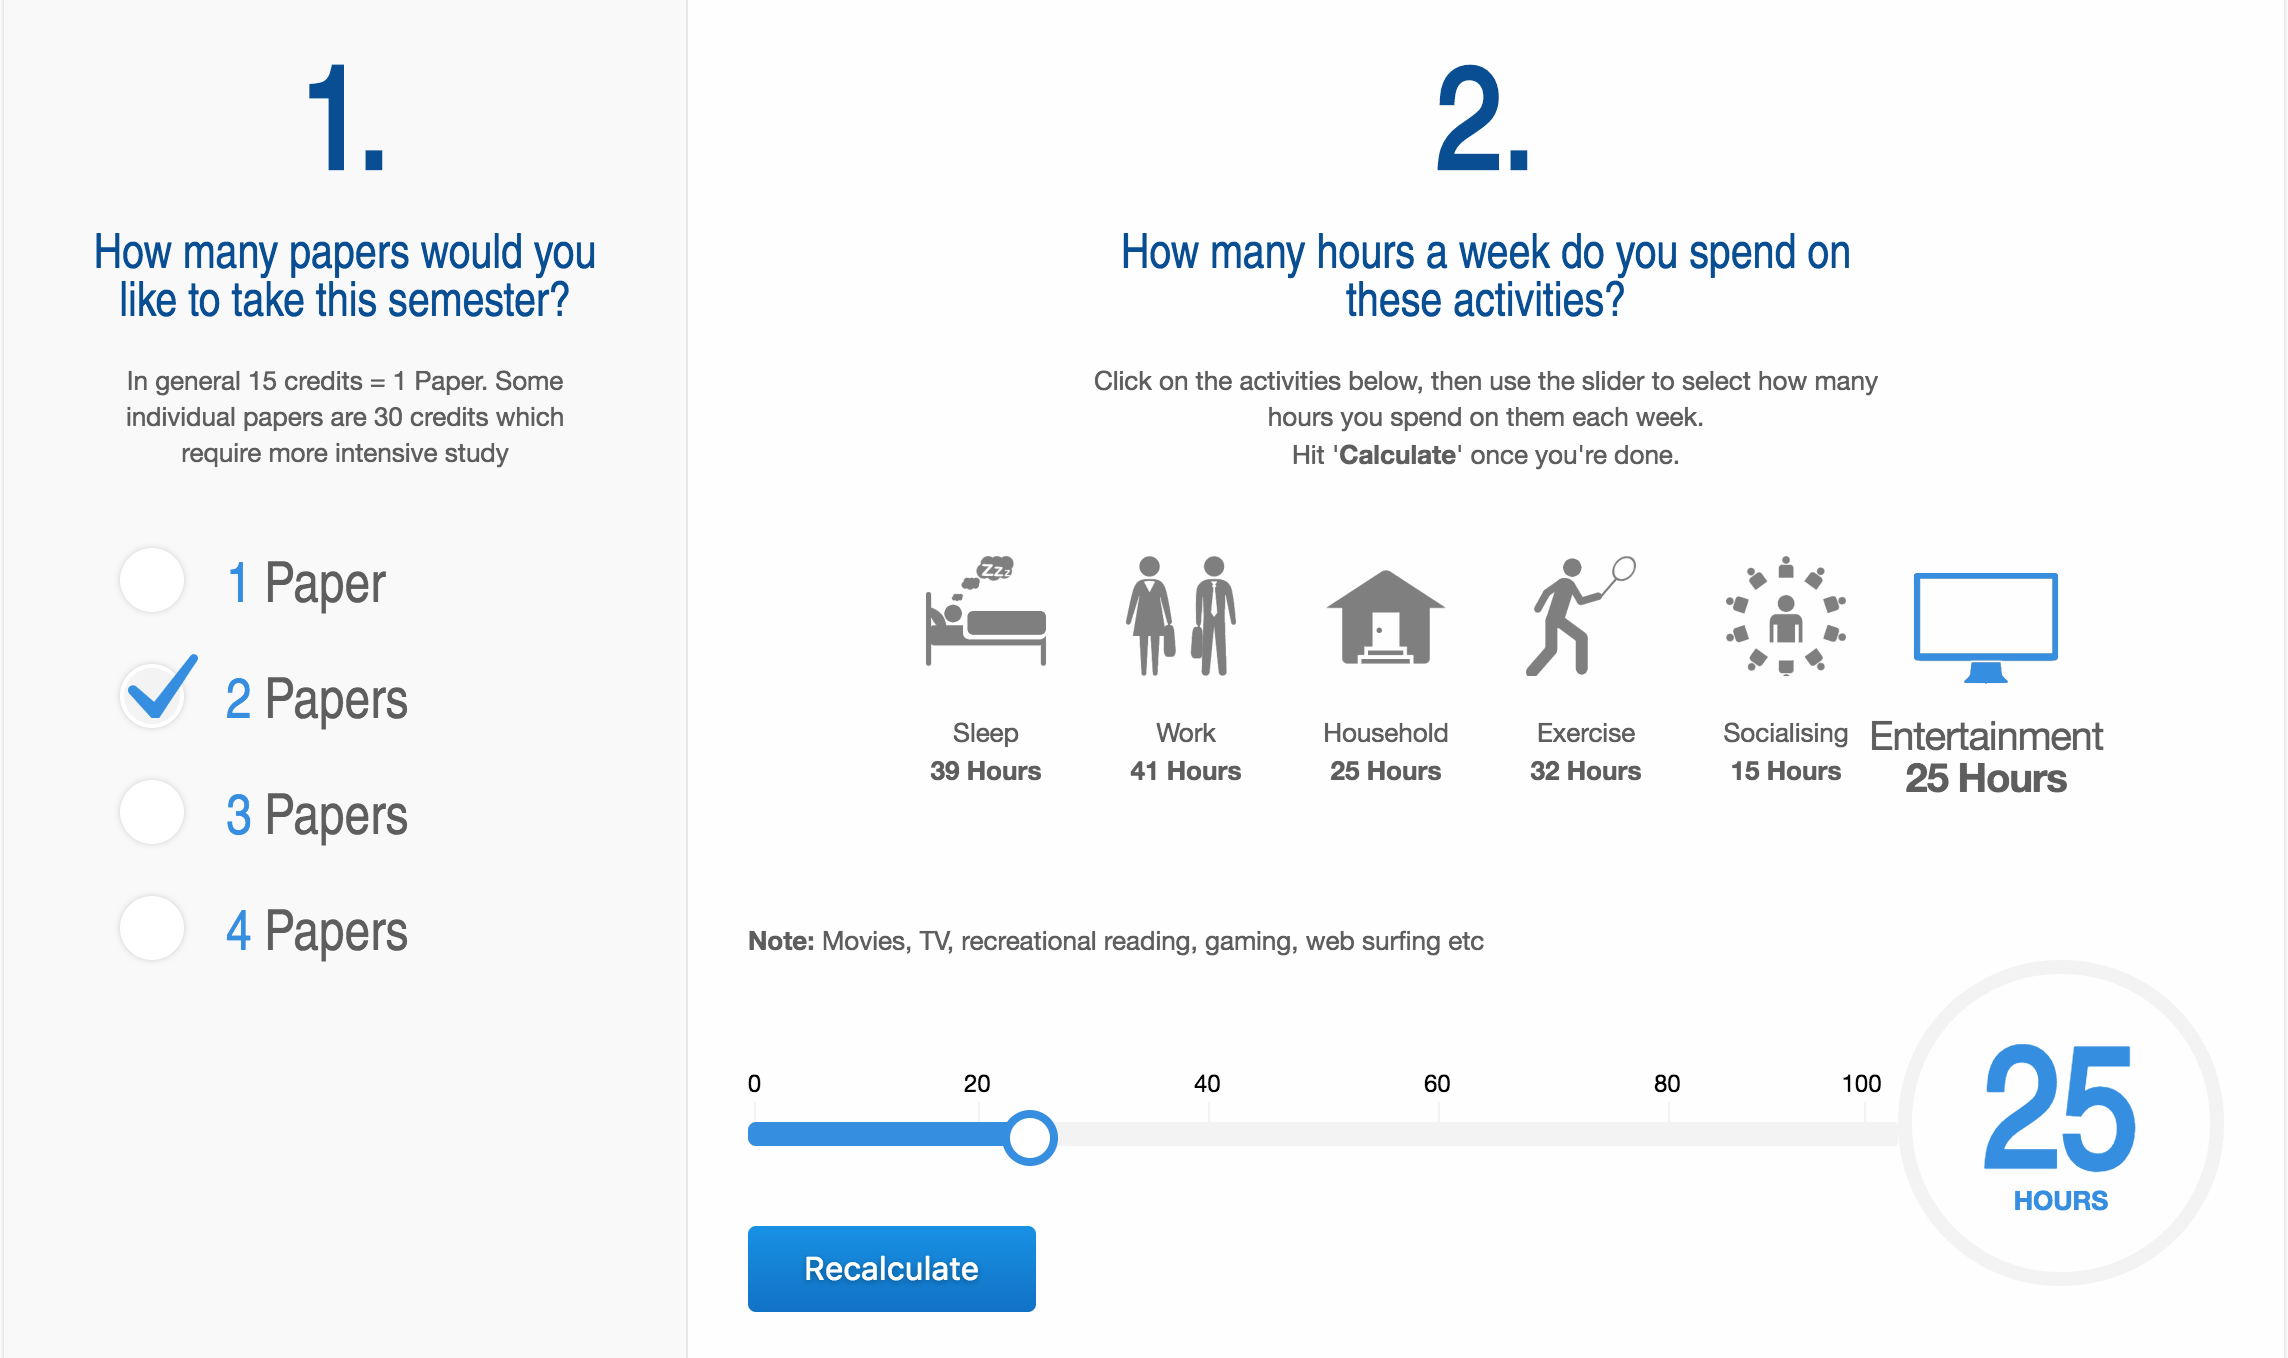
\includegraphics[width=\textwidth]{massey-1}}
\caption{Massey University Workload Planning Tool}
\label{massey-1}
\end{figure}

\begin{figure}
\frame{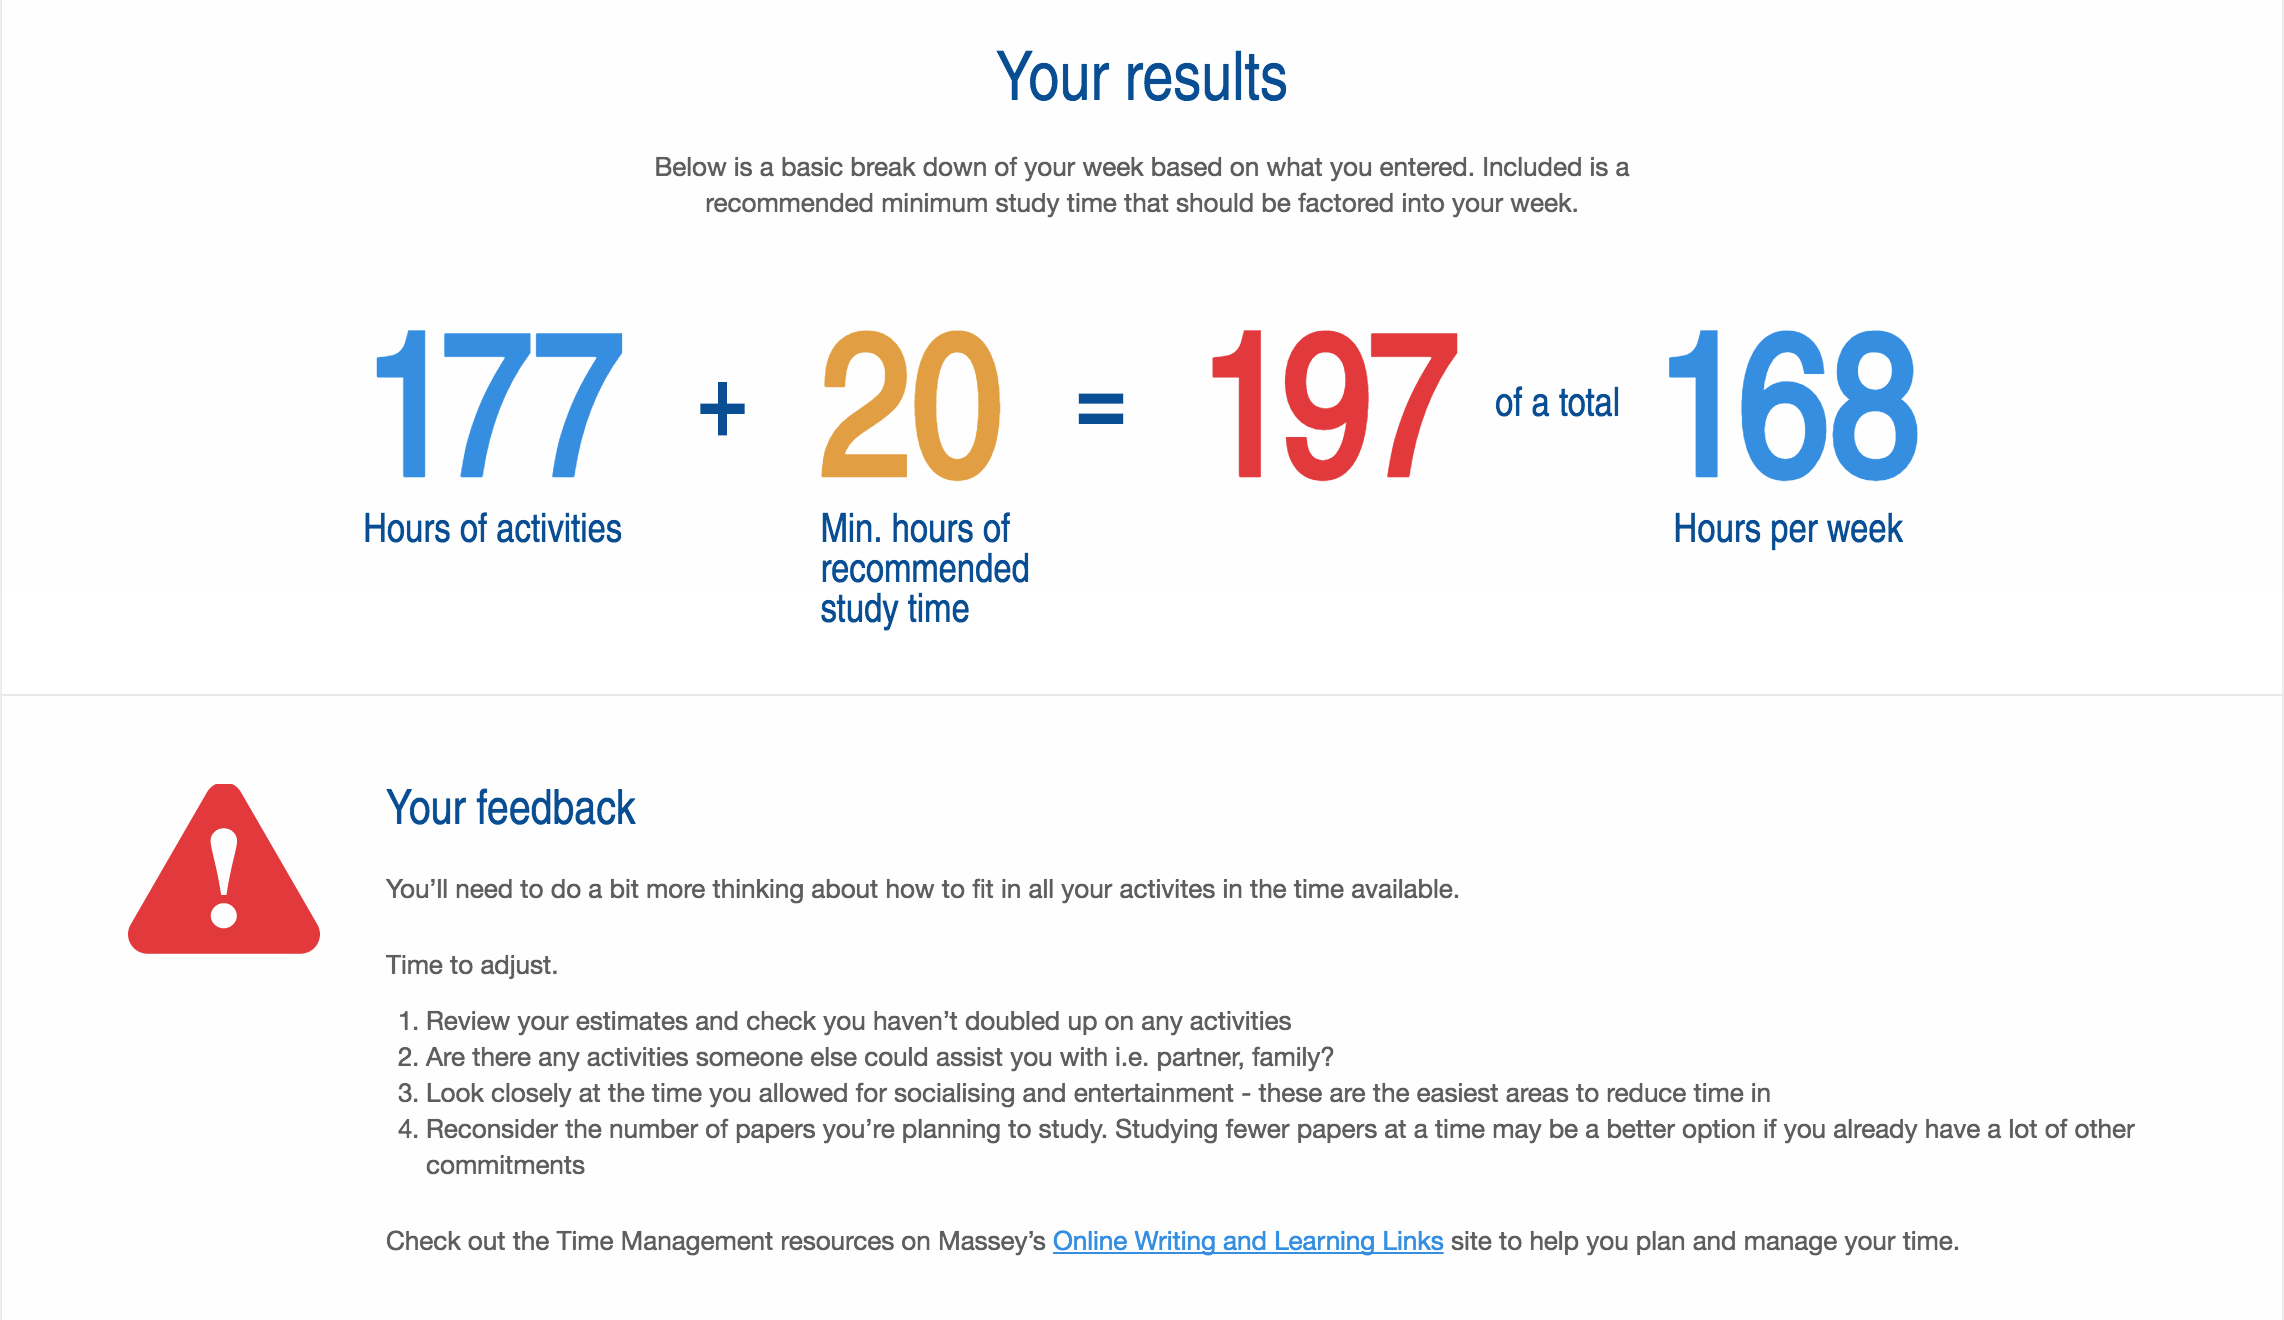
\includegraphics[width=\textwidth]{massey-2}}
\caption{Massey University Workload Planning Tool Result}
\label{massey-2}
\end{figure}

\subsection{An existing workload tool from The Open University}
The second workload is from The Open University, and it is mainly for teaching staff to manage their course workload. As a teaching staff, he or she can add a new faculty, add a new institution and add a new user. Besides, it allows teaching staff to add new courses and edit course details including word count, communication time, experiment time for each activity of each unit and so on. Figure {\ref{open-1}} and {\ref{open-2}} are screenshots of this workload tool.

\begin{figure}
\frame{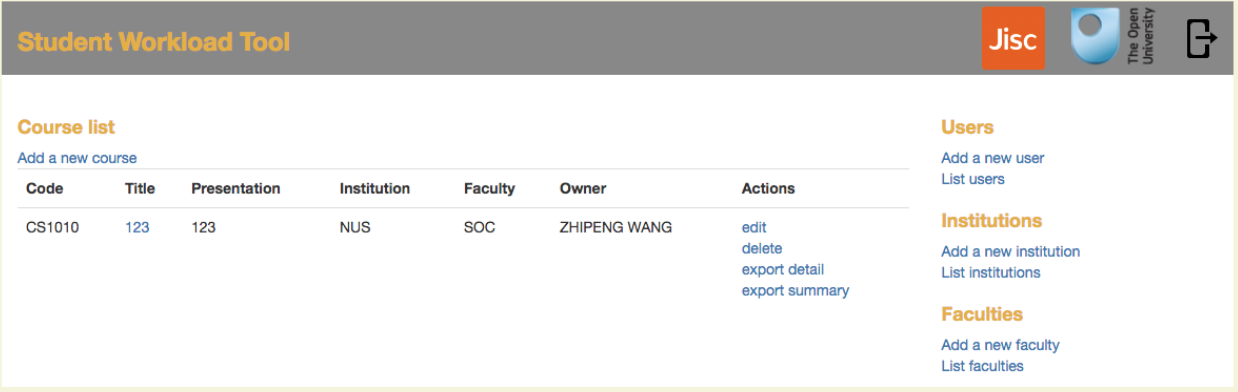
\includegraphics[width=\textwidth]{open-1}}
\caption{Jisc Student Workload Tool (1)}
\label{open-1}
\end{figure}

\begin{figure}
\frame{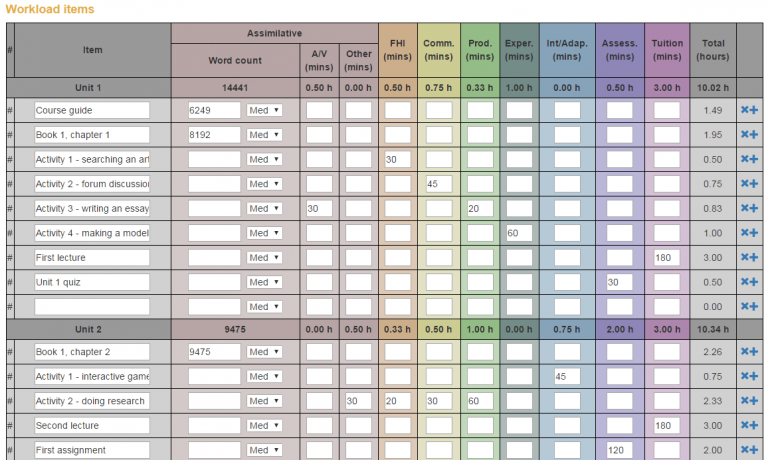
\includegraphics[width=\textwidth]{open-2}}
\caption{Jisc Student Workload Tool (2)}
\label{open-2}
\end{figure}

\chapter{NUSWorks Design}
\section{Introduction}
\subsection{Overview}
NUSWorks is a web-based application that helps NUS undergraduate students easily understand and predict their workload. It uses machine learning algorithm to train the prediction models to make the prediction result become more accurate after being trained with real data. NUS undergraduates can use NUSWorks to predict their future weekly working time for each week and module difficulty based on the provided module details and personal information.

\subsection{Flow}
The Figure {\ref{flow}} shows how the flow of NUSWorks is from user’s perspective.

\begin{figure}
\frame{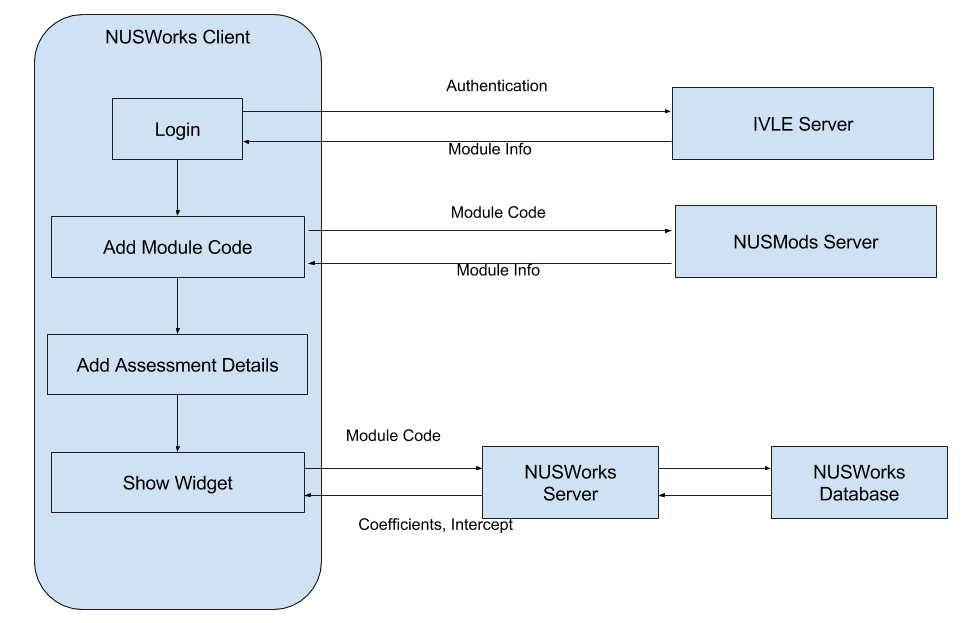
\includegraphics[width=\textwidth]{flow}}
\caption{NUSWorks Flow}
\label{flow}
\end{figure}

\begin{itemize}
  \item Step 1: Users will login via IVLE, and NUSWorks will get the detailed information of the modules that the users have taken through IVLE API after authentication.
  \item Step 2: If users may want to add some modules manually, they can add the module code through the NUSWorks Client and it will fetch the module details through NUSMods API using the module code.
	\item Step 3: Users can choose to add some assessment components of some modules (e.g. add 1 assignment and its details to module CS3219).
	\item Step 4: NUSWorks Client will get the corresponding models from NUSWorks Server and show the predicted results to users (i.e. weekly working time and difficulty) using charts or tables based the information and the models it has.
\end{itemize}

\subsection{Technology stack}
For the front end of NUSWorks, we mainly use React with React-Redux framework. In addition, we use Webpack to package and bundle all the necessary scripts automatically. For the view part, we use React Material UI along with Sass to implement the UI of NUSWorks. Also, we use Yarn package manager to help us maintain the dependencies of Javascript libraries.

For the back end of NUSWorks, we mainly use Flask framework and MariaDB. Also, we use Flask-SQLAlchemy and Flask-Marshmallow to do the communication between server and database. In addition, we use Flask-Restful to build API services for NUSWorks. For the machine learning part, we use scikit-learn library to build and train the machine learning models.

Table {\ref{technology-stack}} shows the summary of technologies used in this project.

\begin{table}[]
\centering
\begin{tabular}{|p{0.35\textwidth}|p{0.65\textwidth}|}
\hline
	\rowcolor[HTML]{C0C0C0}
  \textbf{NUSWorks Client} & \textbf{NUSWorks Server} \\
\hline
ReactJS, React-Redux, Material-UI, Sass, Webpack, Yarn & Flask, MariaDB, scikit-learn, Flask-SQLAlchemy, Flask-Marshmallow, Flask-Restful\\
\hline
\end{tabular}
\caption{NUSWorks Technology Stack Table}
\label{technology-stack}
\end{table}

\section{Model Design}
\subsection{Overview}
For the modelling, we use two indicators to represent student workload which are weekly working time and difficulty. For weekly working time, we build models for each type of assessment for each module. For difficulty, we also build the models for each module.

\subsection{Training system}
\subsubsection{Linear regression algorithm}
For this project, we develop with Linear Regression Algorithm which is one of the simple Machine Learning Algorithms.

For weekly working time, we have separate formula (i.e. Linear Regression Model) for each type of assessment because they should be measured in different ways. For each type of assessment, we use its corresponding training data (i.e. real data from users or volunteers) to train its Linear Regression Model and then use its coefficients and intercept to predict the workload of that assessment for users. For module difficulty, there will be models for each module. The specific attributes of each model will be discussed in 3.2.3 in detail. In addition, for each model (e.g. module difficulty model or assessment model), there will be three levels of complexity: (i) default; (ii) simple; (iii) complex. And the details of each kind of models will be illustrated in 3.2.4 (weekly working time) and 3.2.5 (module difficulty).

For Linear Regression Model, given a random assessment (Y, X1, X2, X3, ...) that Y is the workload of this assessment, and Xi is its related factors. We assume that there might be some linear relationship between Y and Xi, i.e. Y=a1*X1 + a2*X2 + a3*X3 + ... + b. For all training data of (Y, X1, X2, X3, ...), we will find a linear model that fits all training data best among all linear models. To find the most adequate linear model, we could use Least Square Estimation or other estimation techniques. In this project, we use scikit-learn, a Python-based machine learning library, to help us build Ordinary Least Square Linear Regression Models for each type of assessment component or module difficulty of each module.

\subsubsection{Feedback system}
In this project, we allow users to send feedback to the training server containing their actual workload and difficulty (this could be subjective) results if they feel the predicted results are not accurate enough. It is important to build the feedback system because we could know whether the prediction is accurate through the feedback and modify the program or algorithm in time if there are some issues. Also, we could get more real data to train our models. then use the updated model to do prediction after training, and then get feedback again, which forms a feedback cycle that will continuously improve models to make a better prediction.

The main flow of the cycle is shown in the Figure {\ref{training-process}} below. First of all, user can send feedback to the NUSWorks Server if predicted results are inaccurate. Then NUSWorks Server will update the corresponding model and compute the new coefficients and intercept of that model. Next NUSWorks Client will use the new generated model to predict and user still can check and send feedback if necessary.

\begin{figure}
\frame{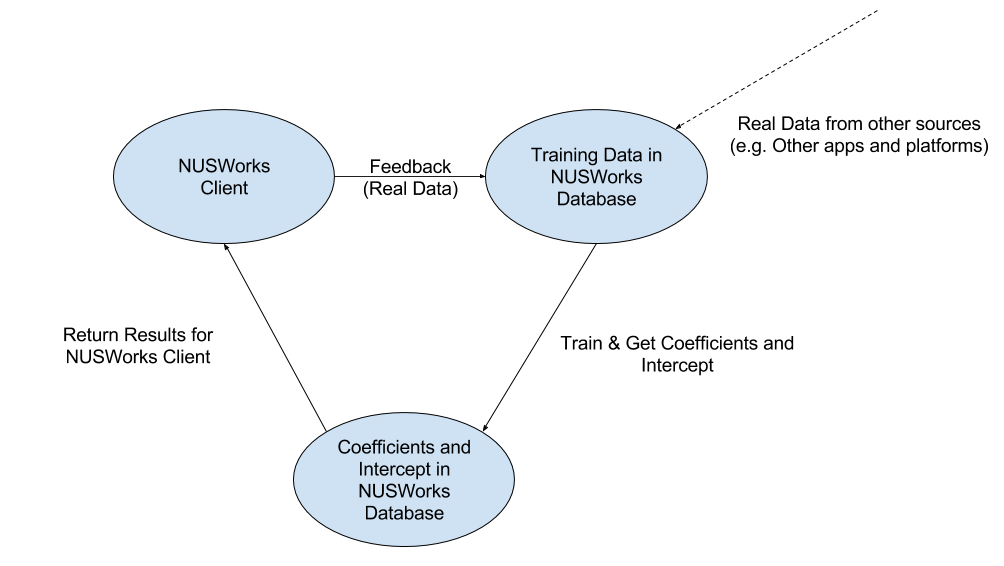
\includegraphics[width=\textwidth]{training-process}}
\caption{NUSWorks Training Process}
\label{training-process}
\end{figure}

\subsubsection{Training data set}
For the training data set of NUSWorks, we could build our own data set by collecting real data from users or volunteers. Also, we can use real data from other apps or platforms to make a larger dataset if possible. However, to integrate others’ dataset, we need to normalise those data before we use it for training.

In addition, we will set a threshold of 20 instances of real data for each model. It means if the size of data set for that model is less than 20 (i.e. less than 20 pieces of real data), the NUSWorks server will not train that model during training process. It is because the predicted results may not be accurate enough if there are too few data for training. Meanwhile, we will cut off the top 5\% and the bottom 5\% data (all the data of each model are sorted by the result field of each piece of real data) to reduce the influence of invalid data.

\subsection{Attributes for models}
\subsubsection{Weekly working time specific attributes}
\begin{itemize}
	\item Assignment specific attributes are shown in Table {\ref{assignment-attribute}}
	\begin{table}[]
	\centering
	\begin{tabular}{|p{0.15\textwidth}|p{0.3\textwidth}|p{0.45\textwidth}|}
	\hline
		\rowcolor[HTML]{C0C0C0}
	  \textbf{Attribute} & \textbf{Definition} & \textbf{Justification} \\
	\hline
	Released week & Starting week of the assignment & Because the app will predict the weekly workload, it can do more precise prediction if exact date is provided \\
	\hline
	Dued week & Ending week of the assignment & Because the app will predict the weekly workload, it can do more precise prediction if exact date is provided \\
	\hline
	Percentage & The percentage of the assignment in the module & Higher percentage can mean more work to be done, which means higher workload \\
	\hline
	Coverage & The amount of lectures the assignment covers & More topics covered could increase the difficulty and preparation time \\
	\hline
	People & The amount of people involved in the assignment & More students involved could increase the difficulty \\
	\hline
	\end{tabular}
	\caption{Assignment Attributes Table}
	\label{assignment-attribute}
	\end{table}

	\item Presentation specific attributes are shown in Table {\ref{presentation-attribute}}
	\begin{table}[]
	\centering
	\begin{tabular}{|p{0.15\textwidth}|p{0.3\textwidth}|p{0.45\textwidth}|}
	\hline
		\rowcolor[HTML]{C0C0C0}
	  \textbf{Attribute} & \textbf{Definition} & \textbf{Justification} \\
	\hline
	Released week & Starting week of the presentation & Because the app will predict the weekly workload, it can do more precise prediction if exact date is provided \\
	\hline
	Dued week & Ending week of the presentation & Because the app will predict the weekly workload, it can do more precise prediction if exact date is provided \\
	\hline
	Percentage & The percentage of the presentation in the module & Higher percentage can mean more work to be done, which means higher workload \\
	\hline
	Coverage & The amount of lectures the presentation covers & More topics covered could increase the difficulty and preparation time \\
	\hline
	People & The amount of people involved in the presentation & More students involved could increase the difficulty \\
	\hline
	Duration & The time duration of the presentation & Longer duration could indicate student need to have a longer preparation time \\
	\hline
	\end{tabular}
	\caption{Presentation Attributes Table}
	\label{presentation-attribute}
	\end{table}

	\item Project specific attributes are shown in Table {\ref{project-attribute}}
	\begin{table}[]
	\centering
	\begin{tabular}{|p{0.15\textwidth}|p{0.3\textwidth}|p{0.45\textwidth}|}
	\hline
		\rowcolor[HTML]{C0C0C0}
	  \textbf{Attribute} & \textbf{Definition} & \textbf{Justification} \\
	\hline
	Released week & Starting week of the project & Because the app will predict the weekly workload, it can do more precise prediction if exact date is provided \\
	\hline
	Dued week & Ending week of the project & Because the app will predict the weekly workload, it can do more precise prediction if exact date is provided \\
	\hline
	Percentage & The percentage of the project in the module & Higher percentage can mean more work to be done, which means higher workload \\
	\hline
	Coverage & The amount of lectures the project covers & More topics covered could increase the difficulty and preparation time \\
	\hline
	People & The amount of people involved in the project & More students involved could increase the difficulty \\
	\hline
	Duration & The time duration of the project & Longer duration could indicate student need to have a longer preparation time \\
	\hline
	\end{tabular}
	\caption{Project Attributes Table}
	\label{project-attribute}
	\end{table}

	\item Reading specific attributes are shown in Table {\ref{reading-attribute}}
	\begin{table}[]
	\centering
	\begin{tabular}{|p{0.15\textwidth}|p{0.3\textwidth}|p{0.45\textwidth}|}
	\hline
		\rowcolor[HTML]{C0C0C0}
	  \textbf{Attribute} & \textbf{Definition} & \textbf{Justification} \\
	\hline
	Amount & The amount of readings measured by how many A4 pages & More amount of readings means it takes more time to finish reading \\
	\hline
	\end{tabular}
	\caption{Reading Attributes Table}
	\label{reading-attribute}
	\end{table}

	\item Test specific attributes are shown in Table {\ref{test-attribute}}
	\begin{table}[]
	\centering
	\begin{tabular}{|p{0.15\textwidth}|p{0.3\textwidth}|p{0.45\textwidth}|}
	\hline
		\rowcolor[HTML]{C0C0C0}
	  \textbf{Attribute} & \textbf{Definition} & \textbf{Justification} \\
	\hline
	Percentage & The percentage of the test in the module & Higher percentage can mean more work to be done, which means higher workload \\
	\hline
	Coverage & The amount of lectures the test covers & More topics covered could increase the difficulty and preparation time \\
	\hline
	Duration & The time duration of the test & Longer duration could indicate student need to have a longer preparation time \\
	\hline
	\end{tabular}
	\caption{Test Attributes Table}
	\label{test-attribute}
	\end{table}

	\item Exam specific attributes are shown in Table {\ref{exam-attribute}}
	\begin{table}[]
	\centering
	\begin{tabular}{|p{0.15\textwidth}|p{0.3\textwidth}|p{0.45\textwidth}|}
	\hline
		\rowcolor[HTML]{C0C0C0}
	  \textbf{Attribute} & \textbf{Definition} & \textbf{Justification} \\
	\hline
	Percentage & The percentage of the exam in the module & Higher percentage can mean more work to be done, which means higher workload \\
	\hline
	Coverage & The amount of lectures the exam covers & More topics covered could increase the difficulty and preparation time \\
	\hline
	Duration & The time duration of the exam & Longer duration could indicate student need to have a longer preparation time \\
	\hline
	\end{tabular}
	\caption{Exam Attributes Table}
	\label{exam-attribute}
	\end{table}
\end{itemize}
\subsubsection{Module difficulty specific attributes}
Module difficulty specific attributes are shown in Table {\ref{difficulty-attribute}}
\begin{table}[]
\centering
\begin{tabular}{|p{0.15\textwidth}|p{0.3\textwidth}|p{0.45\textwidth}|}
\hline
	\rowcolor[HTML]{C0C0C0}
	\textbf{Attribute} & \textbf{Definition} & \textbf{Justification} \\
\hline
Level & The level of the module (e.g. the level of CS3219 is 3) & High level modules should be more difficulty \\
\hline
MC & The modular credits of the module & More modular credits should indicate higher difficulty \\
\hline
Lecture & The number of hours of lecture spent per week & It is one of the related attributes of the module \\
\hline
Tutorial & The number of hours of tutorial spent per week & It is one of the related attributes of the module \\
\hline
Lab & The number of hours of lab spent per week & It is one of the related attributes of the module \\
\hline
Project & The number of hours of project spent per week & It is one of the related attributes of the module \\
\hline
Preparation & The number of hours of preparation per week & It is one of the related attributes of the module \\
\hline
\end{tabular}
\caption{Module Difficulty Attributes Table}
\label{difficulty-attribute}
\end{table}

\subsubsection{Other attributes of student}
It is not enough that we only use module related attributes to compute workload (weekly working time and difficulty in this project) because student ability and effort could also influence the workload (Bowyer, 2012). However, it may not be so easy to measure such attributes like ability and effort. Thus, we have covered some attributes that are student related and may indicate student ability and effort to some extent. The included attributes are shown in the Table {\ref{other-attribute}}.

\begin{table}[]
\centering
\begin{tabular}{|p{0.15\textwidth}|p{0.3\textwidth}|p{0.45\textwidth}|}
\hline
	\rowcolor[HTML]{C0C0C0}
	\textbf{Attribute} & \textbf{Definition} & \textbf{Justification} \\
\hline
CAP & The cumulative average point (CAP) of the student & This may be able to indicate the ability of student \\
\hline
Experienced MC & The amount of modular credits the student has gained & Students have gained more MC seems have a lower workload because they might be more familiar with their major area \\
\hline
Experienced semesters & The number of semesters the student has experienced & Students have gained more semesters seems have a lower workload because they might be more familiar as an undergraduate in NUS \\
\hline
\end{tabular}
\caption{Other Attributes Table}
\label{other-attribute}
\end{table}

\subsection{Weekly working time model for each of the assessment component}
For weekly working time, we have three levels of prediction for each type of assessment. The three levels are (i) default model, (ii) simple model and (iii) complex model. For both (ii) and (iii), we will use linear regression algorithm to build the models based on the training data provided. Also, we have considered assignment, presentation, project, reading, test and exam as assessment components while formulating the model.

\subsubsection{Default model of weekly working time}
For default models of weekly working time for each of the assessment components , we use default models to predict them. We do not use machine learning to refine the models. The default models for each type of assessment are:
\begin{itemize}
	\item \textit{\textbf{Assignment} = weeks * (coverage / 2) * people * (percentage / 5)}
	\item \textit{\textbf{Presentation} = weeks * (coverage / 2) * (people / 4) * (percentage / 5) * duration}
	\item \textit{\textbf{Project} = (weeks / 2) * coverage * (people / 4) * (percentage / 10)}
	\item \textit{\textbf{Reading} = pages / 4}
	\item \textit{\textbf{Test} = (percentage / 10) * coverage * duration}
	\item \textit{\textbf{Exam} = (percentage / 10) * coverage * duration}
\end{itemize}

The “\textit{weeks}” is calculated by \textit{(released week - due week + 1)}.

\subsubsection{Simple model of weekly working time}
For the simple models for weekly working time, it uses linear regression models to predict weekly working time and it will use machine learning to refine the models. The simple models for each type of assessment are:
\begin{itemize}
	\item \textit{\textbf{Assignment} = LRM(weeks, coverage, people, percentage)}
	\item \textit{\textbf{Presentation} = LRM(weeks, coverage, people, percentage, duration)}
	\item \textit{\textbf{Project} = LRM(weeks, coverage, people, percentage)}
	\item \textit{\textbf{Reading} = LRM(pages)}
	\item \textit{\textbf{Test} = LRM(percentage, coverage, duration)}
	\item \textit{\textbf{Exam} = LRM(percentage, coverage, duration)}
\end{itemize}

The “\textit{LSM}” refers to linear regression model, and the attributes inside the parentheses are the required attributes that are provided by users. The “\textit{weeks}” is calculated by \textit{(released week - due week + 1)}.

\subsubsection{Complex model of weekly working time}
For the complex models for weekly working time, it also uses linear regression models to predict weekly working time and it will use machine learning to refine the modes. The difference between simple models and complex models is that complex models are integrated with more attributes (i.e. cumulative average point (CAP), experienced modular credits (MC) and experienced semesters). The complex models for each type of assessment are:
\begin{itemize}
	\item \textit{\textbf{Assignment} = LRM(CAP, experienced MC, experienced semesters, weeks, coverage, people, percentage)}
	\item \textit{\textbf{Presentation} = LRM(CAP, experienced MC, experienced semesters, weeks, coverage, people, percentage, duration)}
	\item \textit{\textbf{Project} = LRM(CAP, experienced MC, experienced semesters, weeks, coverage, people, percentage)}
	\item \textit{\textbf{Reading} = LRM(CAP, experienced MC, experienced semesters, pages)}
	\item \textit{\textbf{Test} = LRM(CAP, experienced MC, experienced semesters, percentage, coverage, duration)}
	\item \textit{\textbf{Exam} = LRM(CAP, experienced MC, experienced semesters, percentage, coverage, duration)}
\end{itemize}

The “\textit{LSM}” refers to linear regression model, and the attributes inside the parentheses are the required attributes that are provided by users. The “\textit{weeks}” is calculated by \textit{(released week - due week + 1)}.

\subsection{Module difficulty model}
For the difficulty, we also build three levels of models to predict difficulty. The three levels are (i) default model, (ii) simple model and (iii) complex model. For both (ii) and (iii), we will use linear regression algorithm to build the models based on the training data provided.

\subsubsection{Default model of module difficulty}
For the default model for difficulty, we simply use the level of the module. For example, for the module CS3219, the difficulty should be 3. The default model represented as formula is:
\begin{itemize}
	\item \textit{\textbf{Module Difficulty} = level + (mc - 4) / 4}
\end{itemize}

When the size of training data set is not large enough (i.e. less than 20 instances of real data for one type of assessment component of one module), we will use the default models. Otherwise, we will use simple models or complex models.

\subsubsection{Simple model of module difficulty}
For the simple model for module difficulty, we build a linear regression model to predict the module difficulty. The simple model is:
\begin{itemize}
	\item \textit{\textbf{Module Difficulty} = LRM(level, mc, lecture, tutorial, lab, project, preparation)}
\end{itemize}

The “\textit{LSM}” refers to linear regression model, and the attributes inside the parentheses are the required attributes that are provided by users or IVLE.

\subsubsection{Complex model of module difficulty}
For the complex model for module difficulty, we also build a linear regression model to predict the module difficulty. The difference between simple model and complex model of difficulty is that complex model is integrated with more attributes (i.e. cumulative average point (CAP), experienced modular credits (MC) and experienced semesters). The complex model for module difficulty is:
\begin{itemize}
	\item \textit{\textbf{Module Difficulty} = LRM(CAP, experienced MC, experienced semesters, level, mc, lecture, tutorial, lab, project, preparation)}
\end{itemize}

The “\textit{LSM}” refers to linear regression model, and the attributes inside the parentheses are the required attributes that are provided by users or IVLE.

\section{Features}
\subsection{Predict weekly working time based on information provided}
NUSWorks can accept various amount of information from student to generate predicted weekly working time. For example, a student can only add modules in NUSWorks without any assessment components and a prediction result will also be generated based on the modules themselves. If more information is provided, such as some assessment components, the result will be more accurate because it will use the corresponding model to calculate the weekly working time for that assessment component and add it to the final total weekly working time.

For the models used to predict weekly working time, if there are not more than 20 instances of real training data for that type of assessment component of that module, then we will use default model of that assessment component of that module. Otherwise, user can choose either use simple models or complex models

\subsection{Predict module difficulty based on information provided}
NUSWorks can accept various amount of information from student to generate predicted module difficulty. For example, a student can add modules in NUSWorks and a predicted module difficulty for each module will be generated based on the modules themselves. If more information is provided, such as student CAP, experienced MC and experienced semesters, the result will be more accurate because it will use the corresponding model to compute the predicted difficulty for that module.

For the model used to predict module difficulty, if there are not more than 20 instances of real training data for that module, then we will use default model of that module to predict module difficulty. Otherwise, user can choose either use simple model or complex model to predict module difficulty.

\subsection{Different ways to visualise prediction results}
Users can choose preferred ways to show the predicted result. For weekly working time, user can choose to show the predicted result as a line chart, or a bar chart, or a pie chart, or just a table.

\subsection{Feedback system of prediction}
Users can send feedback to NUSWorks training server if the prediction results are not accurate and the feedback will be stored as real data into the database. Then the feedback data will be used in the next training round for the corresponding model for refinement.

\section{Requirements}
\subsection{Functional requirements}
\begin{itemize}
	\item A student should be able to login via IVLE and all the needed information should be fetched automatically.
	\item A student should be able to manually add, edit and delete module information besides fetching information from IVLE.
	\item A student should be able to add, edit, delete assignment, project, presentation, reading, test, exam details of each added module.
	\item A student should be able to view the charts and tables that contain the prediction results.
	\item System should be able to generate the corresponding charts and tables if minimum required inputs has been entered, and more accurate results should be computed out if more details provided.
	\item A student should be able to view all the information he or she has entered and all the charts and tables has been shown if the student reopen the application.
	\item A student should be able to send feedback to the training server if the predicted results are not accurate.
	\item System should be able to generate the linear regression models for predicting weekly working time and difficulty of each module from training data set.
	\item System should be able refine and update the linear regression models by training the models with real data and feedback data.
\end{itemize}

\subsection{Non-functional requirements}
\begin{itemize}
	\item Response time should be short, which is less than 1 second.
	\item System should be easily mastered by students.
	\item Module information from back end should be consistent with IVLE.
	\item System should be easily maintained and extended if continuous development needed.
	\item System should handle both valid and invalid input and response correspondingly.
	\item Database should be backuped in case need to restore when data loss.
\end{itemize}

\section{Design Decisions}
\subsection{Architecture}
\subsubsection{NUSWorks Client}
Because I use React-Redux as the framework for the front end of NUSWorks, so the architecture of the front end flows the Redux design, and Figure {\ref{redux}} shows the flow of Redux while using React together.

\begin{figure}
\frame{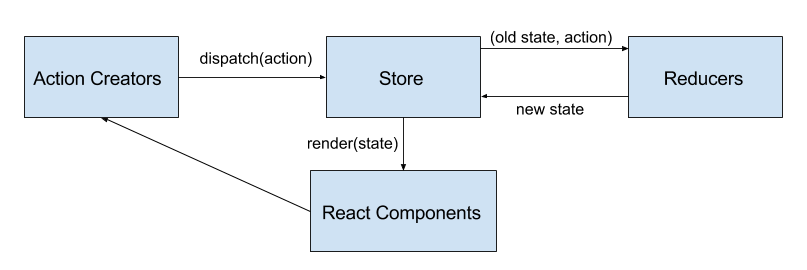
\includegraphics[width=\textwidth]{redux}}
\caption{React-Redux Flow}
\label{redux}
\end{figure}

There are four main kinds of components including Action Creators, Store, Reducers and React Components.

\begin{itemize}
	\item React Component: React Component is more like customised HTML tags, and it mainly deals with for the view part of application.
	\item Store: Store is to store the state of whole application, and it maintains a storage tree that every time it will replace the partial state with its new state.
	\item Action Creator: Action Creator is to create action objects that are used as parameter of dispatch function.
	\item Reducer: Reducer is to create new state according to the old state and action.
\end{itemize}

Every time there is a user request that may lead to changing of views, React Components will call corresponding Action Creator to request the action object, and then use the dispatch function, provided by Store, to emit the action to Store. Then Store will call the corresponding Reducer to return back the new state by using the old state and action object. Finally, after Store updates the state and re-render the corresponding React Components using updated state.

Redux is good at maintaining the status of components. Also, there is only one data store, which will ensure the data consistency. In addition, the data in the store can be easily passed to any components via its connect method. Meanwhile, because there are a lot of situations in this project that components need to sharing data and status, and one component may change the states of other components, it is simple and convenient to achieve them using Redux rather than other architectures.

\subsubsection{NUSWorks Server}
For the backend of NUSWorks, I use the Flask to set up the NUSWorks server. The NUSWorks server currently will provide API services for NUSWorks app. The API services including getting coefficients and intercept of some linear regression model of some assessment component or module difficulty of some module and posting real data (e.g. user feedback) for training. The main architecture of NUSWorks server is shown in the Figure {\ref{nusworks-server}}.

\begin{figure}
\frame{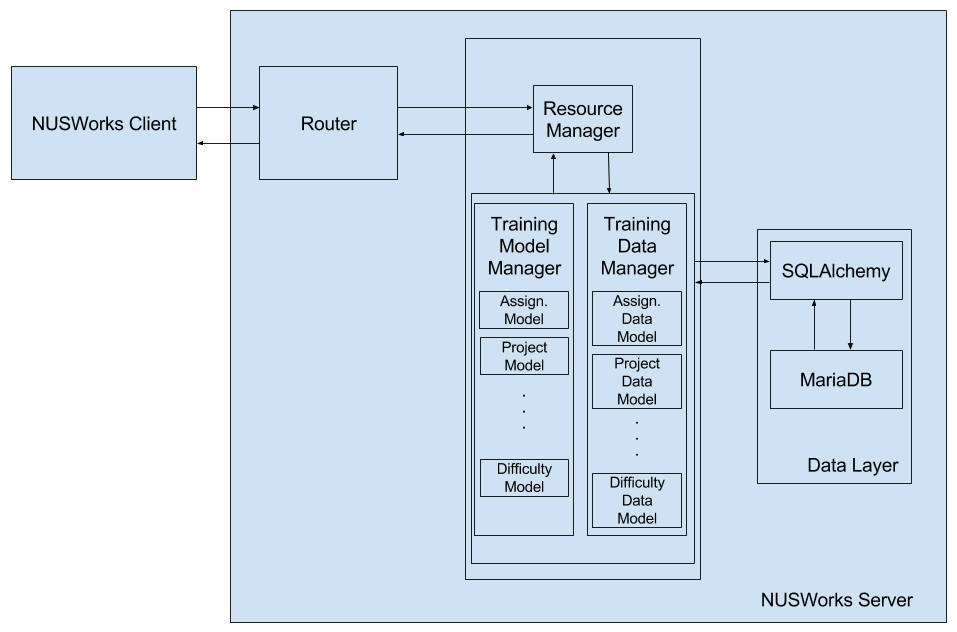
\includegraphics[width=\textwidth]{nusworks-server}}
\caption{NUSWorks Server Flow}
\label{nusworks-server}
\end{figure}

Initially, once NUSWorks client makes a request, the router will parse the request URL and determine which resource is requested by the client. If the request is to get the coefficients and intercept of some model, then the corresponding model (e.g. Project Model) will fetch its coefficients and intercept from NUSWorks Database through SQLAlchemy; if the request is to add training data to database, then its corresponding data model (e.g. Project Data Model) will send the data to NUSWorks Database through SQLAlchemy.

Flask is a lightweight framework compared to other Python frameworks. Since the NUSWorks Server may only deal with the requests from the NUSWorks Client and we do not need other functionalities, Flask is enough and it is easy to set it up. Besides, Object Relational Mapping is applied (i.e. Flask-SQLAlchemy and Flask-Marshmallow) to deal with the communications between NUSWorks Server and NUSWorks Database.

\subsection{UI/UX Design}
Since we use Material-UI in this project, all the UI design follows material design.
\begin{itemize}
	\item Initially, Figure {\ref{screen-1}} the user interface while first time opening NUSWorks.
	\item If top left button is clicked, a drawer window will pop out from left side which contains the modules that the user has added to NUSWorks (Shown in Figure {\ref{screen-2}}).
	\item If bottom right button in the drawer window is clicked, a new window will pop out and user can add new modules to NUSWorks (Shown in Figure {\ref{screen-3}}).
	\item Autocompletion for module is implemented for convenience (Shown in Figure {\ref{screen-4}}).
	\item If one of the module in the module list is clicked, user can view the details of that module which includes all the assessment information of that module. Each tab represents one kind of assessment. User can add, edit or delete assessment information for all the modules (Shown in Figure {\ref{screen-5}}).
	\item If the close button of one module is clicked, that module will be removed from NUSWorks.
	\item If top right button is clicked, the browser will be redirected to IVLE login page. After login via IVLE account, it will be redirected back to NUSWorks. In addition, all the modules in IVLE will be imported to NUSWorks automatically as well as some personal information of the user (e.g. name, matriculation number), and some of the tables and charts has been generated based on the imported modules. This will reduce the preparation work that the user has to do before viewing the results.
	\item The top right button has been changed to a menu button (Shown in Figure {\ref{screen-6}}). If it is clicked, a menu containing three options will pop out (Shown in Figure {\ref{screen-7}}).
	\item If “Profile” option is selected, a small window will pop out in the center of browser. The window contains some personal information of the user which is got from IVLE. Besides, some input fields are provided for user to enter some information that may be used for prediction. Once “OK” button is clicked, the information entered will be stored (Shown in Figure {\ref{screen-8}}).
	\item If “Feedback” option is selected, a small window will pop out in the center of browser. The window contains some input fields and each input field is related to one predicted result. User can enter the actual value if the predicted result is not accurate, and keep it empty if it is accurate. Once “Send” is clicked, all the feedbacks will be sent to the NUSWorks Server and they might be used as training data for next training process (Shown in Figure {\ref{screen-9}}).
	\item If “Logout” option is selected, the current session will be closed and all the information imported from the user’s IVLE account should be cleared. Also, the top right button will also be changed to “LOGIN” button.
	\item For each tab on the left side, it represents one table or chart that will show the information of current workload. User can move the mouse over the tabs to know the name of each tab.
	\item If the first tab (i.e. time table tab) is clicked, the time table of the user will be shown (Shown in Figure {\ref{screen-10}}).
	\item User can move the mouse over the occupied square (i.e. squares in purple) to know which module has occupied this time slot (Shown in Figure {\ref{screen-11}}).
	\item If the second tab (i.e. weekly working time table) is clicked, a table that shows the weekly working time of every week of each module will be shown. Each value of weekly working time are generated based on its corresponding model (Shown in Figure {\ref{screen-12}}).
	\item User can select different level of complexity for models (Shown in Figure {\ref{screen-13}}).
	\item If the third tab (i.e. weekly working time line chart) is clicked, a line chart that shows the weekly working time of every week will be shown. It will show the trend of weekly working time either for all the modules or for one specific module. Each value of weekly working time are generated based on its corresponding model (Shown in Figure {\ref{screen-14}}).
	\item User can select one module to view its weekly working time, or select “All” to view the total weekly working time. Also, user can select different level of complexity for models (Shown in Figure {\ref{screen-15}}).
	\item If the fourth tab (i.e. weekly working time bar chart) is clicked, a bar chart that shows the weekly working time of every week will be shown. Each value of weekly working time are generated based on its corresponding model (Shown in Figure {\ref{screen-16}}).
	\item User can select one module to view its weekly working time, or select “All” to view the total weekly working time. Also, user can select different level of complexity for models (Shown in Figure {\ref{screen-17}}).
	\item If the fifth tab (i.e. working time pie chart) is clicked, a pie chart that shows the ratio of total working time of each module (Shown in Figure {\ref{screen-18}}).
	\item If one of the module (i.e. not the “All” selection) is selected, the new pie chart will show the ratio of total working time of each assessment component of that module. “base” part represents the weekly working time provided by IVLE (i.e. lecture, tutorial, lab, project, and preparation) (Shown in Figure {\ref{screen-19}}).
	\item If the sixth tab (i.e. module difficulty table) is clicked, a table that shows the module difficulty information of each module will be shown. User can view the module difficulty generated by simple models and complex models. Meanwhile, User can view the highest and the lowest module difficulty of each module (Shown in Figure {\ref{screen-20}}).
\end{itemize}

\subsection{Testing}
Since testing is not the first priority for this project, and there is limited time, we do not fully test both NUSWorks Client and NUSWorks Server. However, in the future, we must fully test NUSWorks before deploy it online.

Firstly, we use React built-in type checking functionality to handle React components type checking. It allows us to check if the type of value is the same as the specified type, and errors will be thrown if they are not matched.

Besides, we use Mocha and Enzyme to set up our testing framework and write some simple unit tests and integration tests for NUSWorks Client. We have created one unit test for some components in NUSWorks Client, and in each unit test, we have checked whether the current component is correctly rendered and the values are correctly passed to this component. For unit test, we mainly use the shallow method from Enzyme because shallow will only render the first level of nodes, which is fast and efficient. For simple integration test, we use mount method to do integration test because mount method will render all levels of children nodes and components, which is exactly what integration test will do.

\chapter{Discussion and Recommendation}
\section{Machine Learning Model}
In this project, we assume that the relationship between the workload (i.e. weekly working time and module difficulty) and the attributes used in this project is linear, and use linear regression model to predict weekly working time and difficulty. The reason why we use linear regression model is that it is a simple machine learning model that can be easily implemented, and it is the first time to applying machine learning algorithm to education workload prediction.

As mentioned in the introduction part, it is hard to define and measure workload, but also knowing workload is quite important for students. Although we cannot come up with a direct formula to calculate workload manually, we could analyse the real data that might be related to workload to build a model for workload, which is the main idea of machine learning.

However, it may not be linear between the workload, or the weekly working time and module difficulty in this project, and the workload-related attributes, and even more complicated than linear relationship. Thus, we need to do more research on the relationship between the workload and the workload-related attributes, and we have to use another more appropriate model, like artificial neural networks model, rather than linear regression model if the relationship is non linear.

\section{Training Data}
In this project, since we use machine learning algorithm (i.e. linear regression algorithm), we need to collect real data to train our linear regression models. Currently we only have two channels to collect data. One is to collect data from friends or volunteers, the other one is to collect data from other applications or platforms. However, there are still some problems. First of all, the amount of data collected from friends would be limited, and also some data collected from other applications and platforms may miss some attributes or cannot be normalized to the format we need. One way to collect more valid data could be introducing NUSWorks to some lecturers and letting them ask their students to use NUSWorks.

\section{Attributes of Models}
The attributes involved in this project has been introduced in 3.2.3. However, there are still some uninvolved attributes that might be related to workload. For example, teaching approaches, learning environment, and student effort. The reason why we do not cover those attributes is that it is difficulty to define and quantify them. We cannot just use a numeric value to represent teaching approach or learning environment, and more research should be conducted on them before we include those attributes to the workload models. In addition, we should also include more attributes that are workload-related and easily measured to make the workload models more powerful and accurate.

\section{Indicators of Workload}
Currently there are two indicators of workload in this project: (i) weekly working time, and (ii) module difficulty. However, there might still exist more indicators of workload or more appropriate indicators that reveal the student workload more precisely as a replacement of the weekly working time and/or module difficulty. This is related to how we want to define and represent student workload, and how the student workload should be measured. Thus, this could be one of the future extension of this project.

\chapter{Conclusion}
To sum up, in this project, we have studied about what student workload is and how we understand and measure student workload. Meanwhile, to address this problem, we have built several models to represent student workload and used those models to build a tool, NUSWorks, to help NUS undergraduates understand their workload by predicting their weekly working time and module difficulty using machine learning algorithm. However, this project is just a first try to model the student workload and use machine learning to calculate workload based those models, and NUSWorks still has some limitations such as not enough indicators of workload and maybe inappropriate model used.

Meanwhile, this project is an enriching and helpful experience for me because it enhances my web development skills and research skills. Also, it gives me a chance to learn and apply machine learning technology. In addition, I have got deep insight into education system and student workload system during this project. All of these may benefit me in my future career.

\bibliographystyle{socreport}
\bibliography{socreport}

\appendix
\chapter{Screenshots}
\begin{figure}
\frame{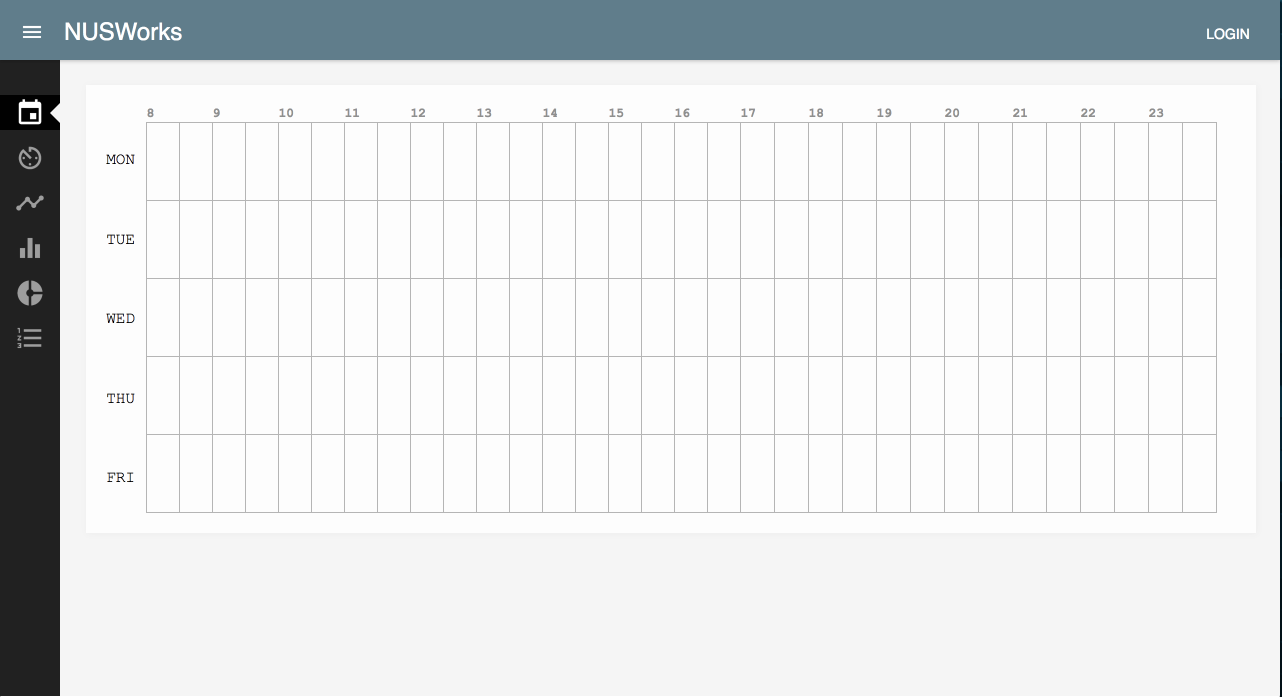
\includegraphics[width=\textwidth]{1}}
\caption{NUSWorks Screenshot (1)}
\label{screen-1}
\end{figure}

\begin{figure}
\frame{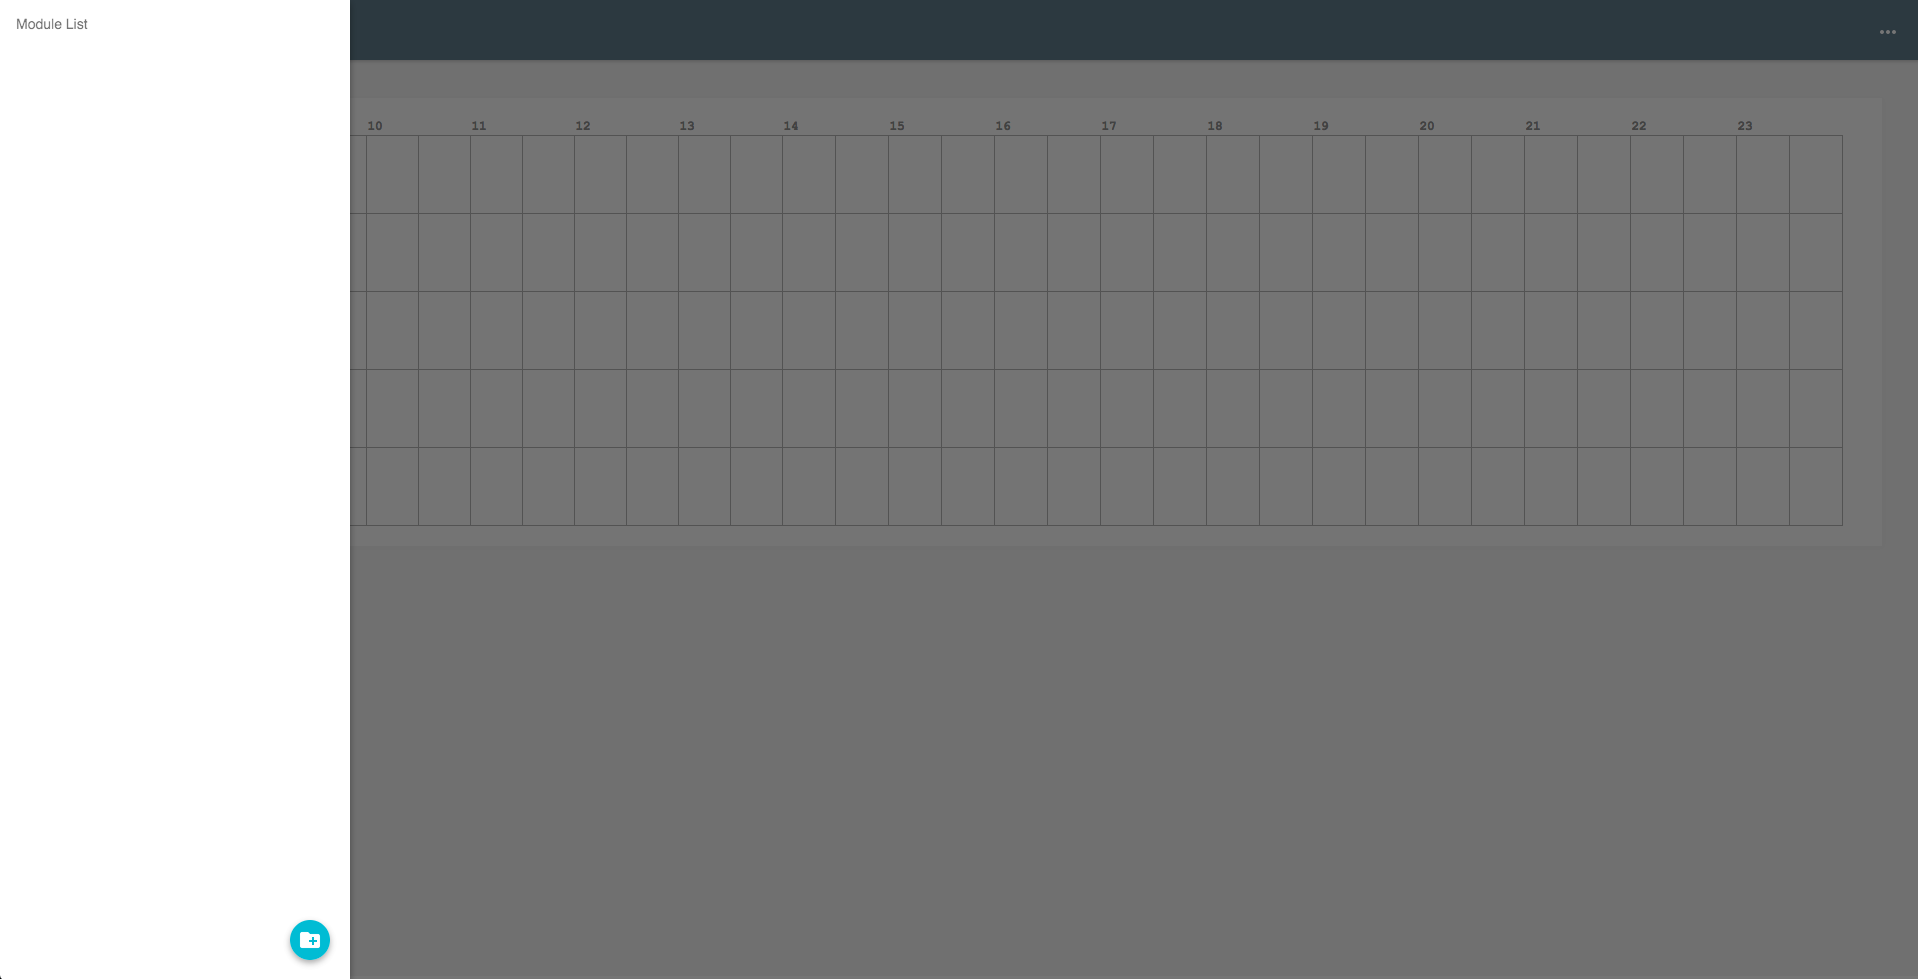
\includegraphics[width=\textwidth]{2}}
\caption{NUSWorks Screenshot (2)}
\label{screen-2}
\end{figure}

\begin{figure}
\frame{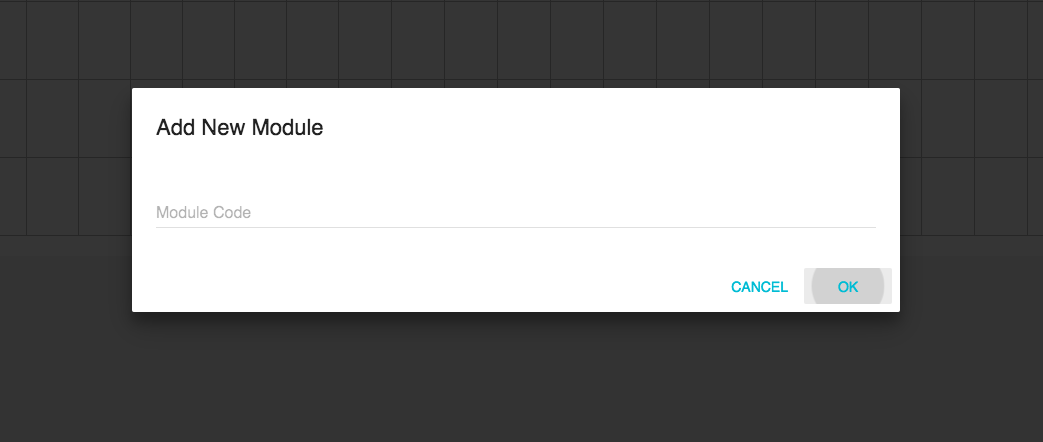
\includegraphics[width=\textwidth]{3}}
\caption{NUSWorks Screenshot (3)}
\label{screen-3}
\end{figure}

\begin{figure}
\frame{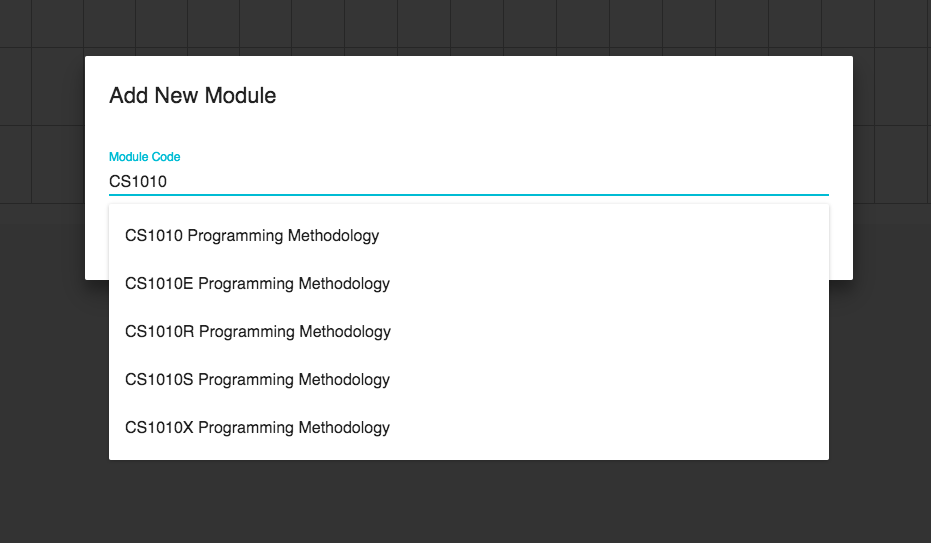
\includegraphics[width=\textwidth]{4}}
\caption{NUSWorks Screenshot (4)}
\label{screen-4}
\end{figure}

\begin{figure}
\frame{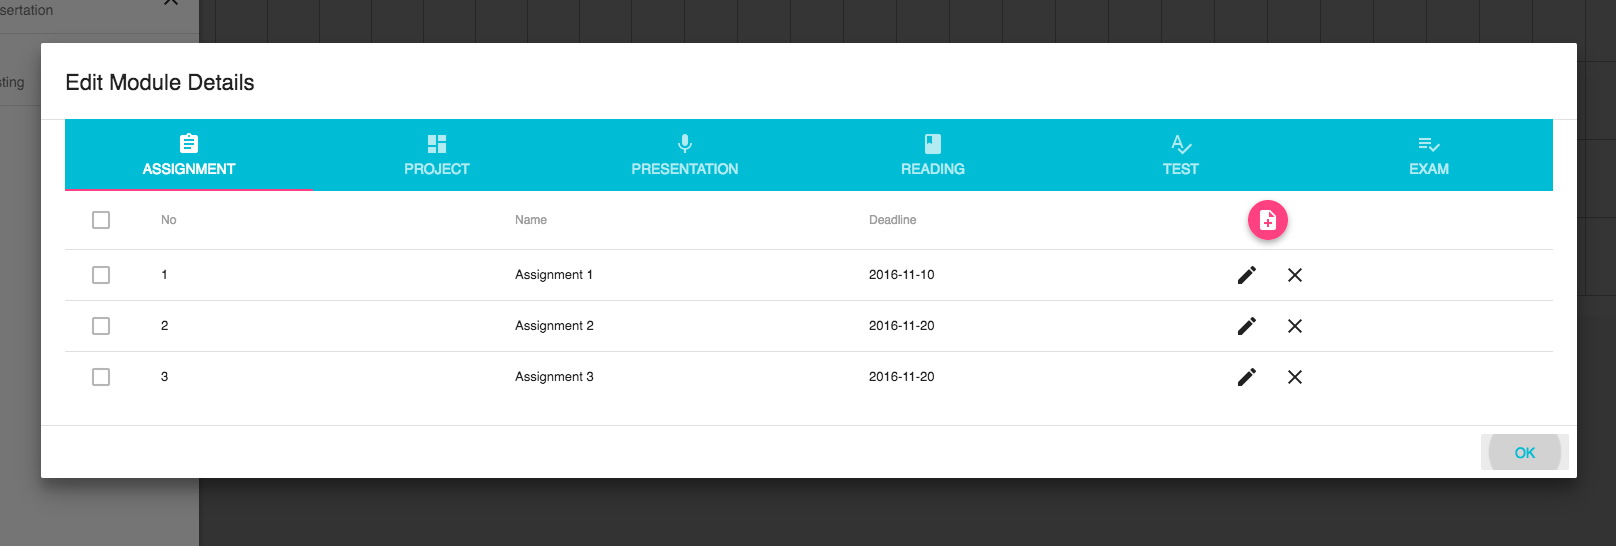
\includegraphics[width=\textwidth]{5}}
\caption{NUSWorks Screenshot (5)}
\label{screen-5}
\end{figure}

\begin{figure}
\frame{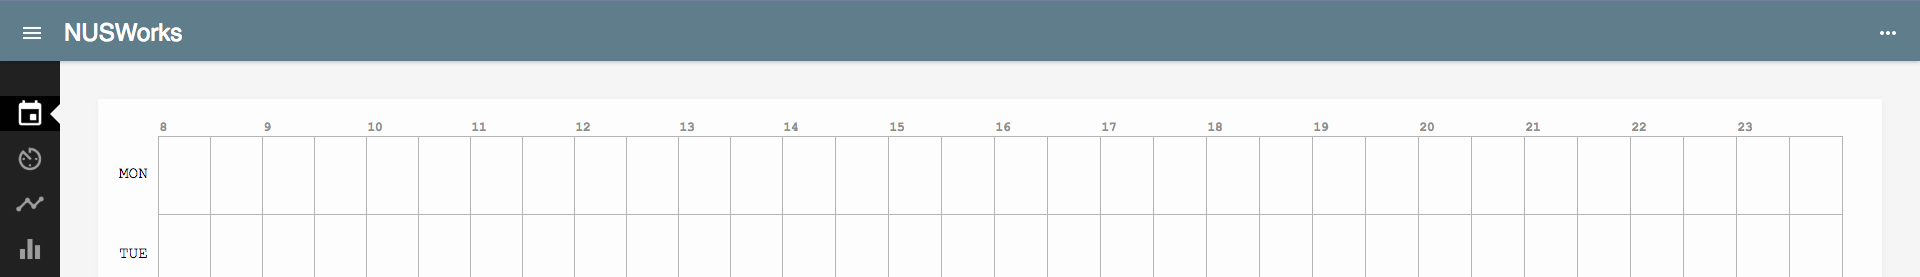
\includegraphics[width=\textwidth]{6}}
\caption{NUSWorks Screenshot (6)}
\label{screen-6}
\end{figure}

\begin{figure}
\frame{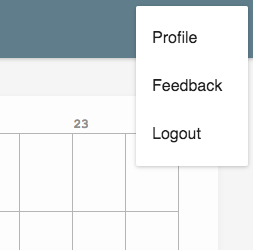
\includegraphics[width=\textwidth]{7}}
\caption{NUSWorks Screenshot (7)}
\label{screen-7}
\end{figure}

\begin{figure}
\frame{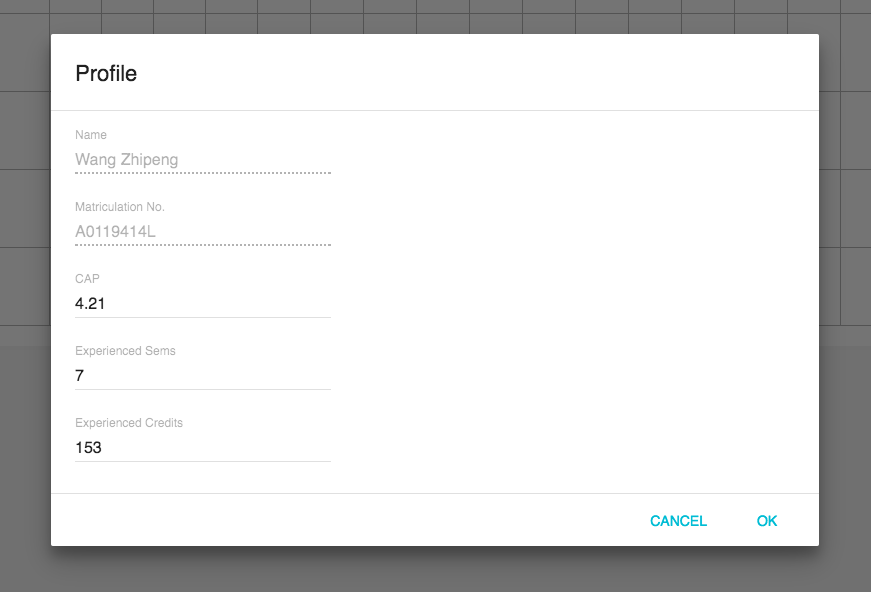
\includegraphics[width=\textwidth]{8}}
\caption{NUSWorks Screenshot (8)}
\label{screen-8}
\end{figure}

\begin{figure}
\frame{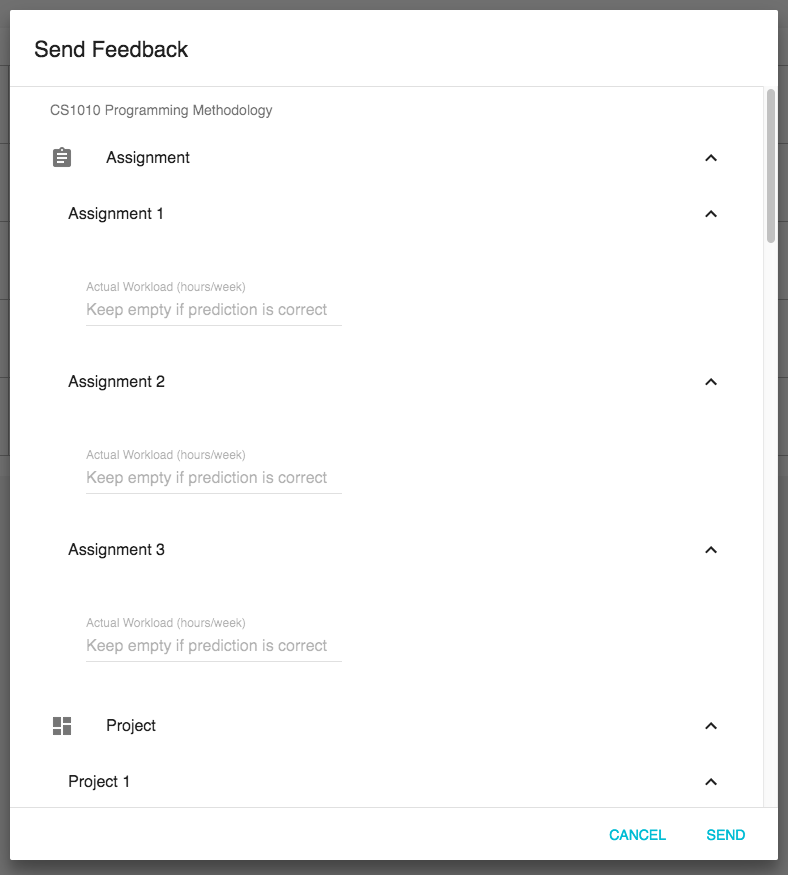
\includegraphics[width=\textwidth]{9}}
\caption{NUSWorks Screenshot (9)}
\label{screen-9}
\end{figure}

\begin{figure}
\frame{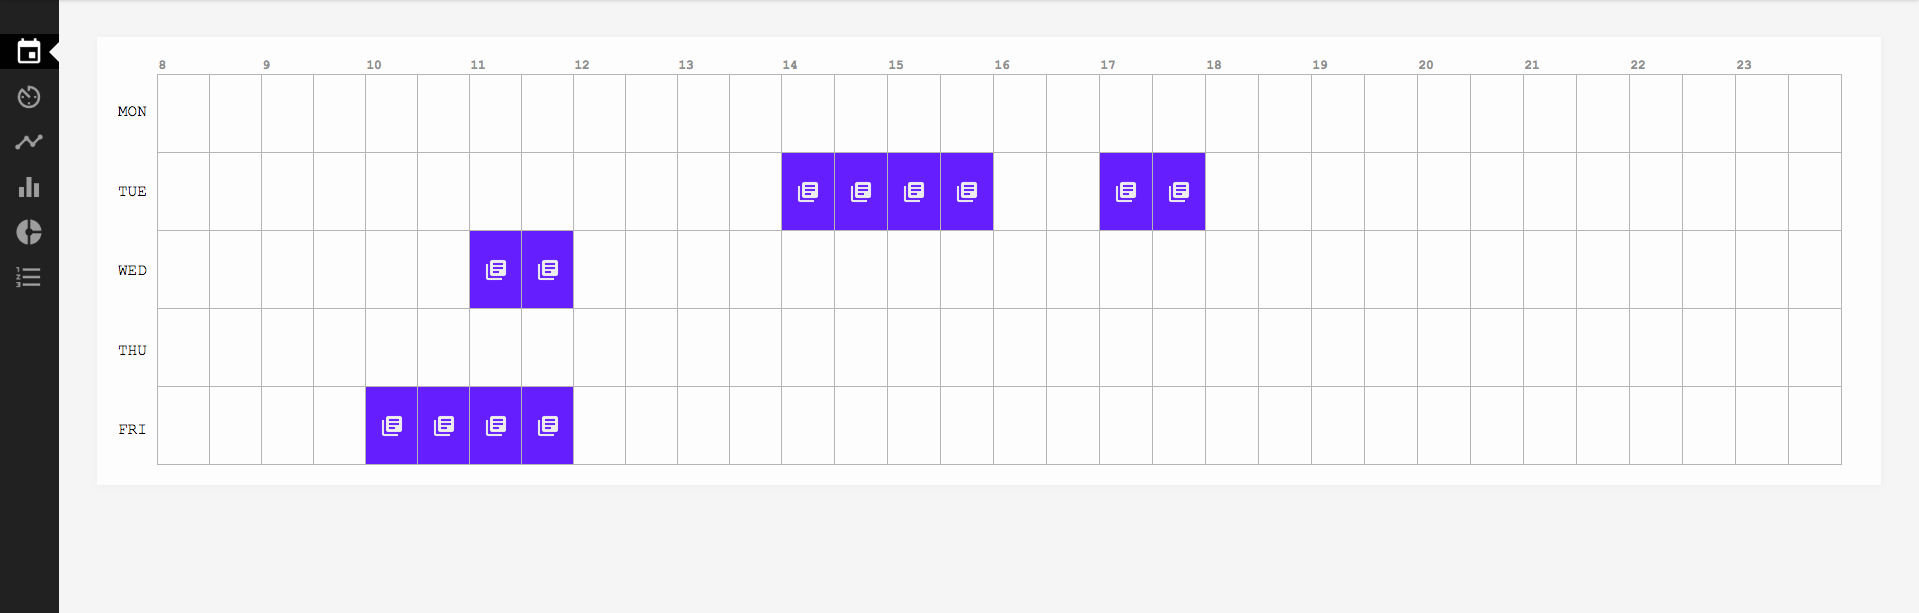
\includegraphics[width=\textwidth]{10}}
\caption{NUSWorks Screenshot (10)}
\label{screen-10}
\end{figure}

\begin{figure}
\frame{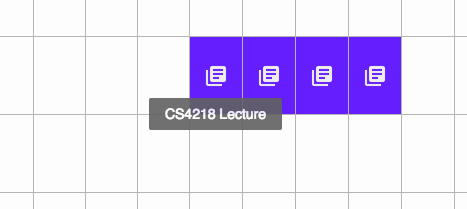
\includegraphics[width=\textwidth]{11}}
\caption{NUSWorks Screenshot (11)}
\label{screen-11}
\end{figure}

\begin{figure}
\frame{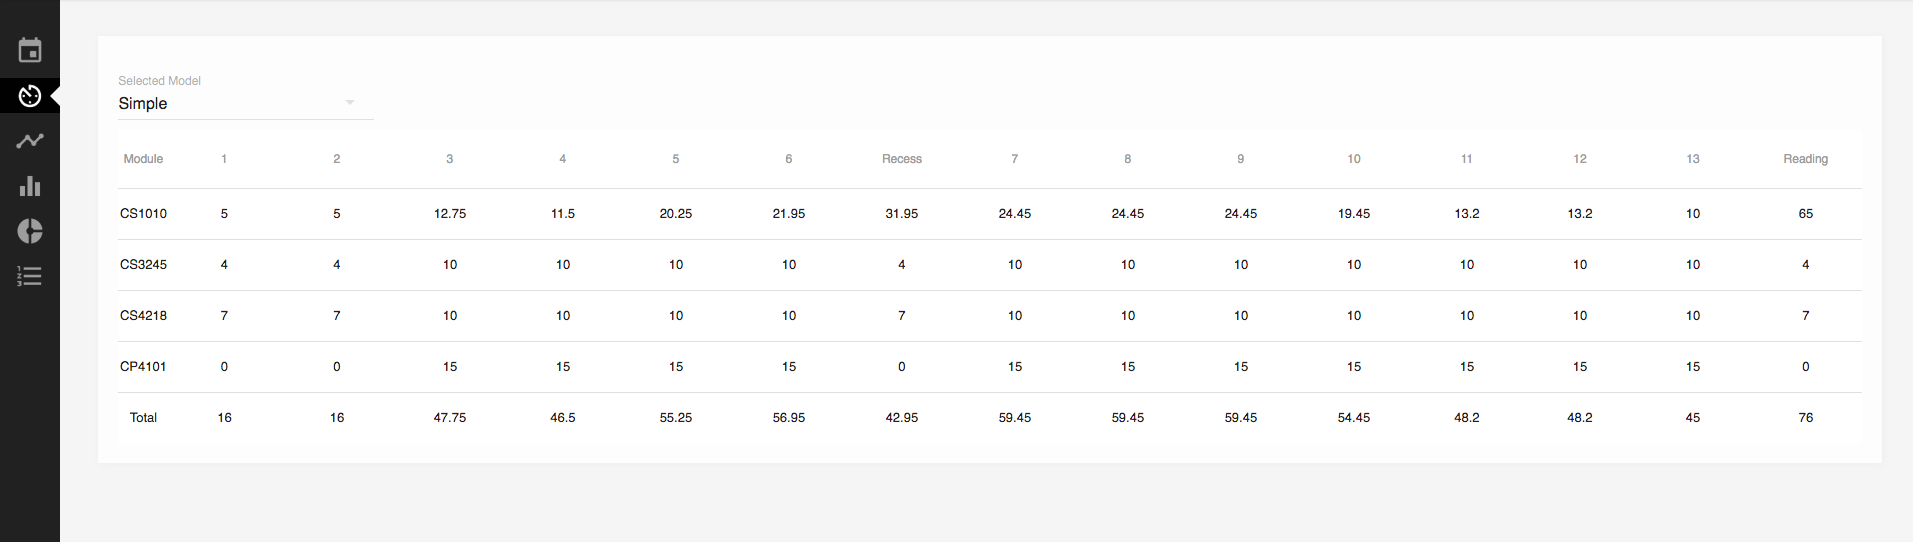
\includegraphics[width=\textwidth]{12}}
\caption{NUSWorks Screenshot (12)}
\label{screen-12}
\end{figure}

\begin{figure}
\frame{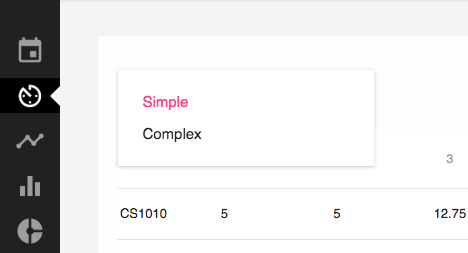
\includegraphics[width=\textwidth]{13}}
\caption{NUSWorks Screenshot (13)}
\label{screen-13}
\end{figure}

\begin{figure}
\frame{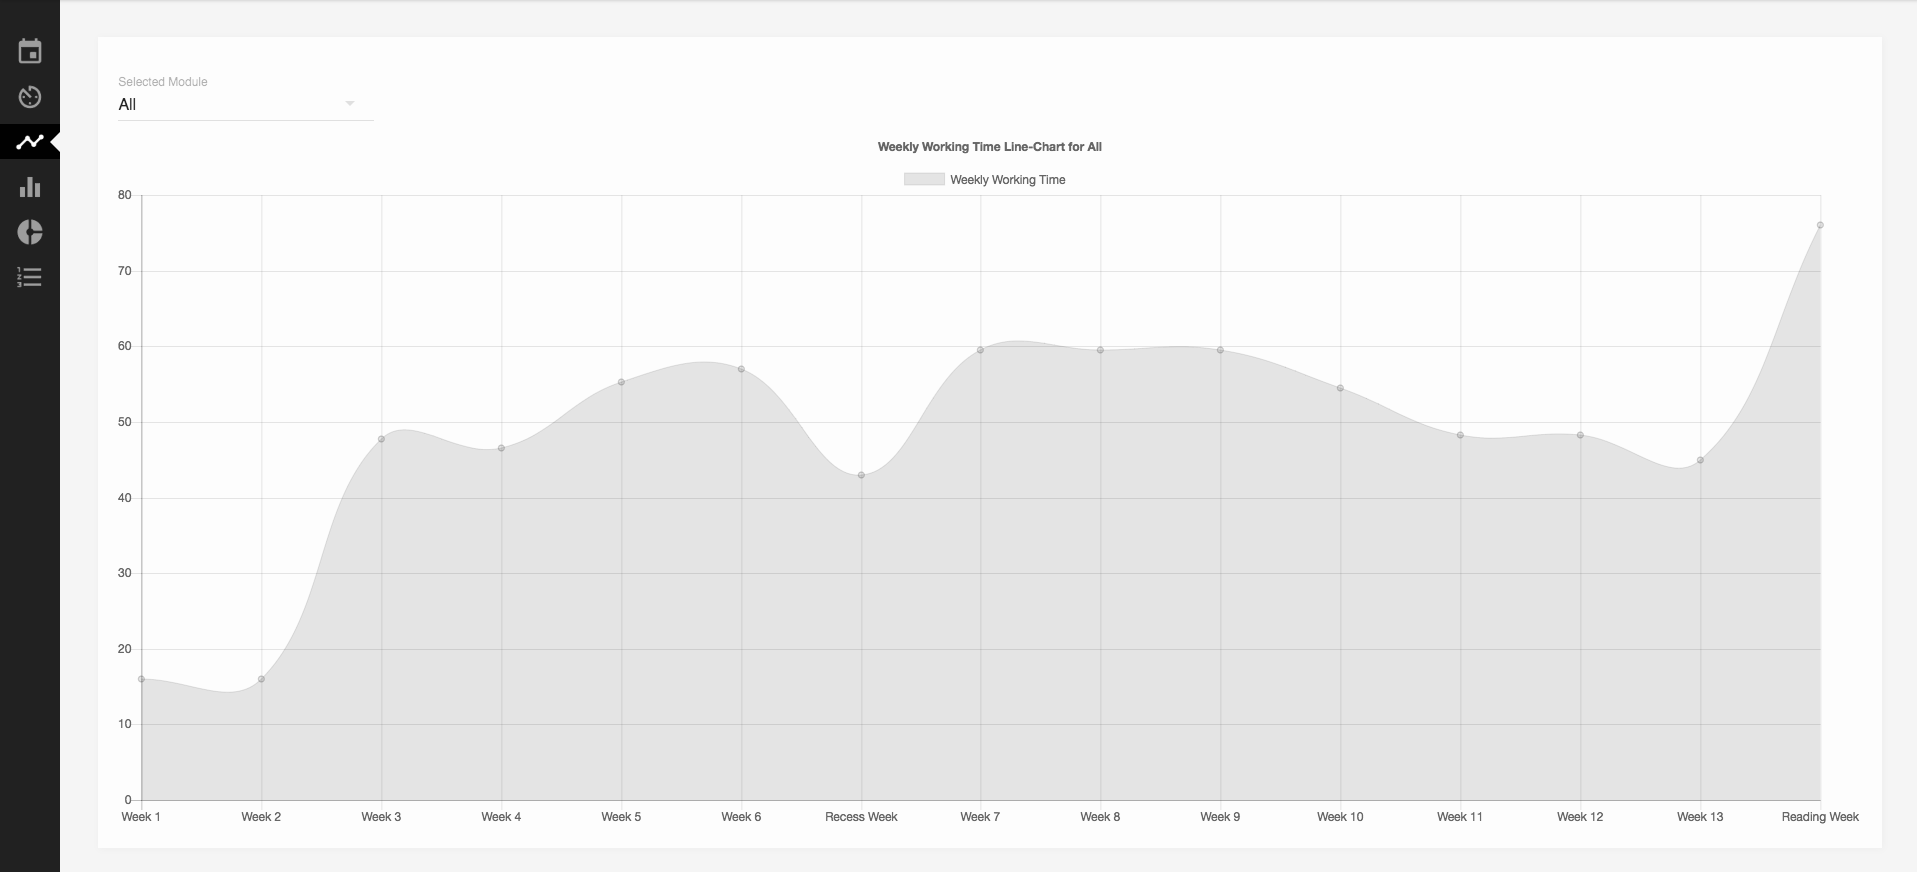
\includegraphics[width=\textwidth]{14}}
\caption{NUSWorks Screenshot (14)}
\label{screen-14}
\end{figure}

\begin{figure}
\frame{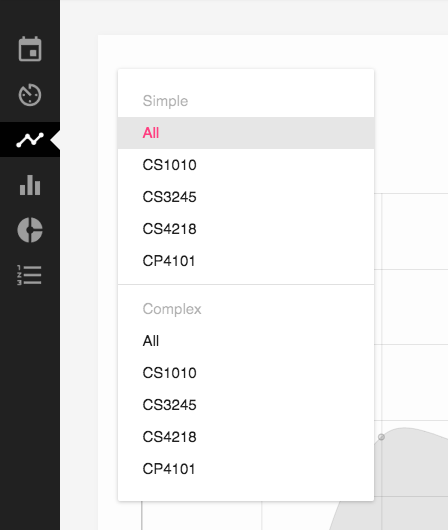
\includegraphics[width=\textwidth]{15}}
\caption{NUSWorks Screenshot (15)}
\label{screen-15}
\end{figure}

\begin{figure}
\frame{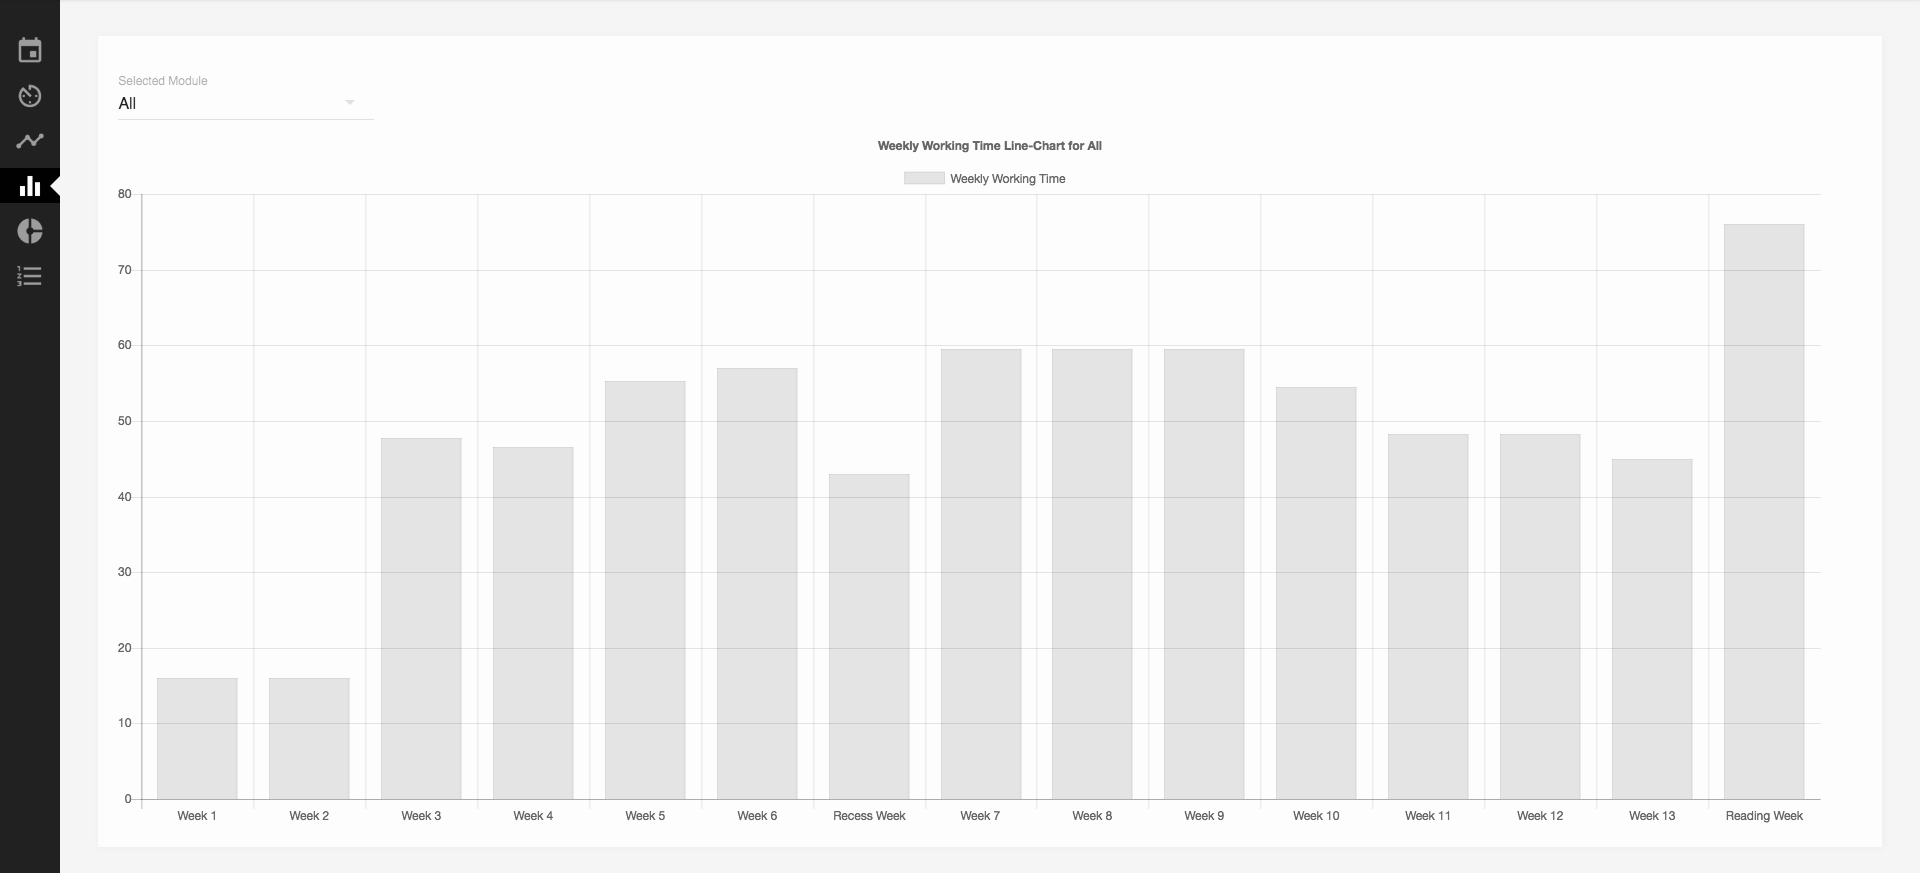
\includegraphics[width=\textwidth]{16}}
\caption{NUSWorks Screenshot (16)}
\label{screen-16}
\end{figure}

\begin{figure}
\frame{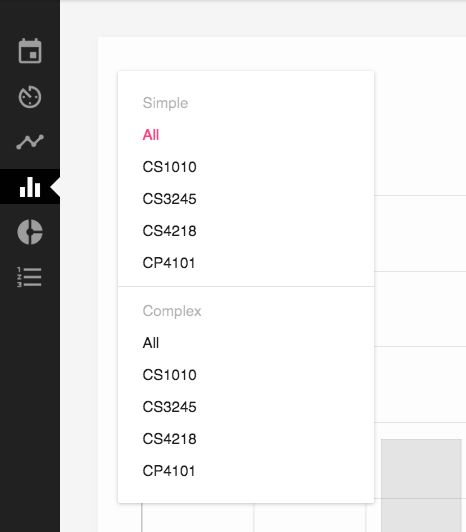
\includegraphics[width=\textwidth]{17}}
\caption{NUSWorks Screenshot (17)}
\label{screen-17}
\end{figure}

\begin{figure}
\frame{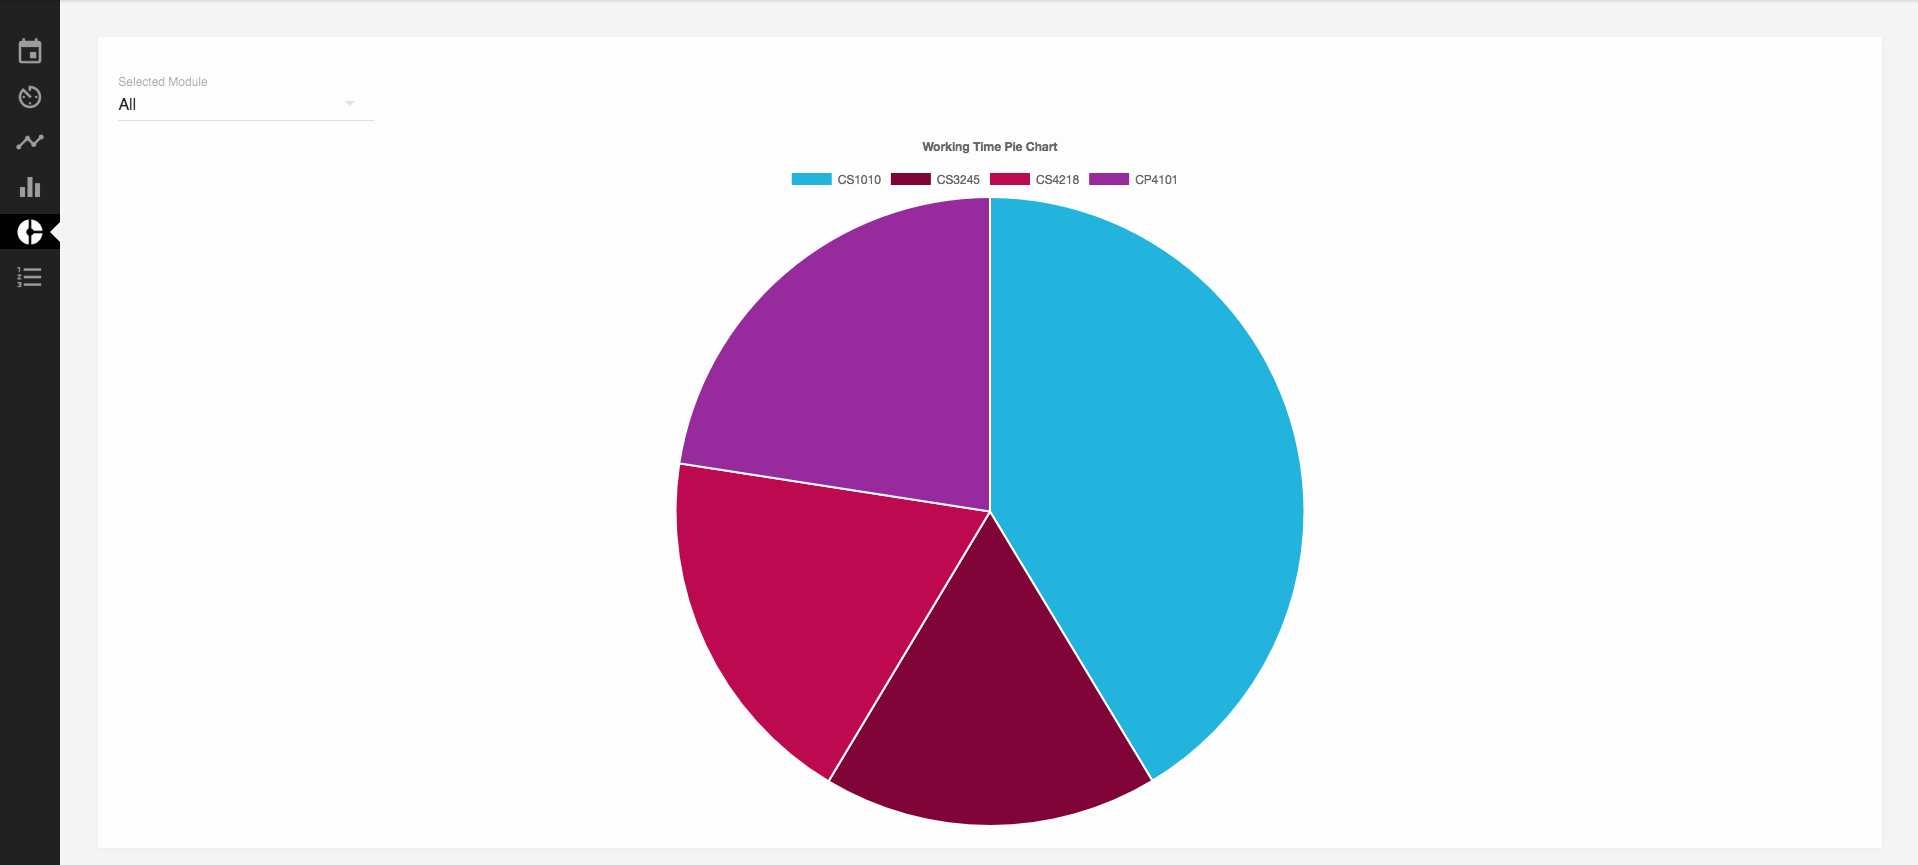
\includegraphics[width=\textwidth]{18}}
\caption{NUSWorks Screenshot (18)}
\label{screen-18}
\end{figure}

\begin{figure}
\frame{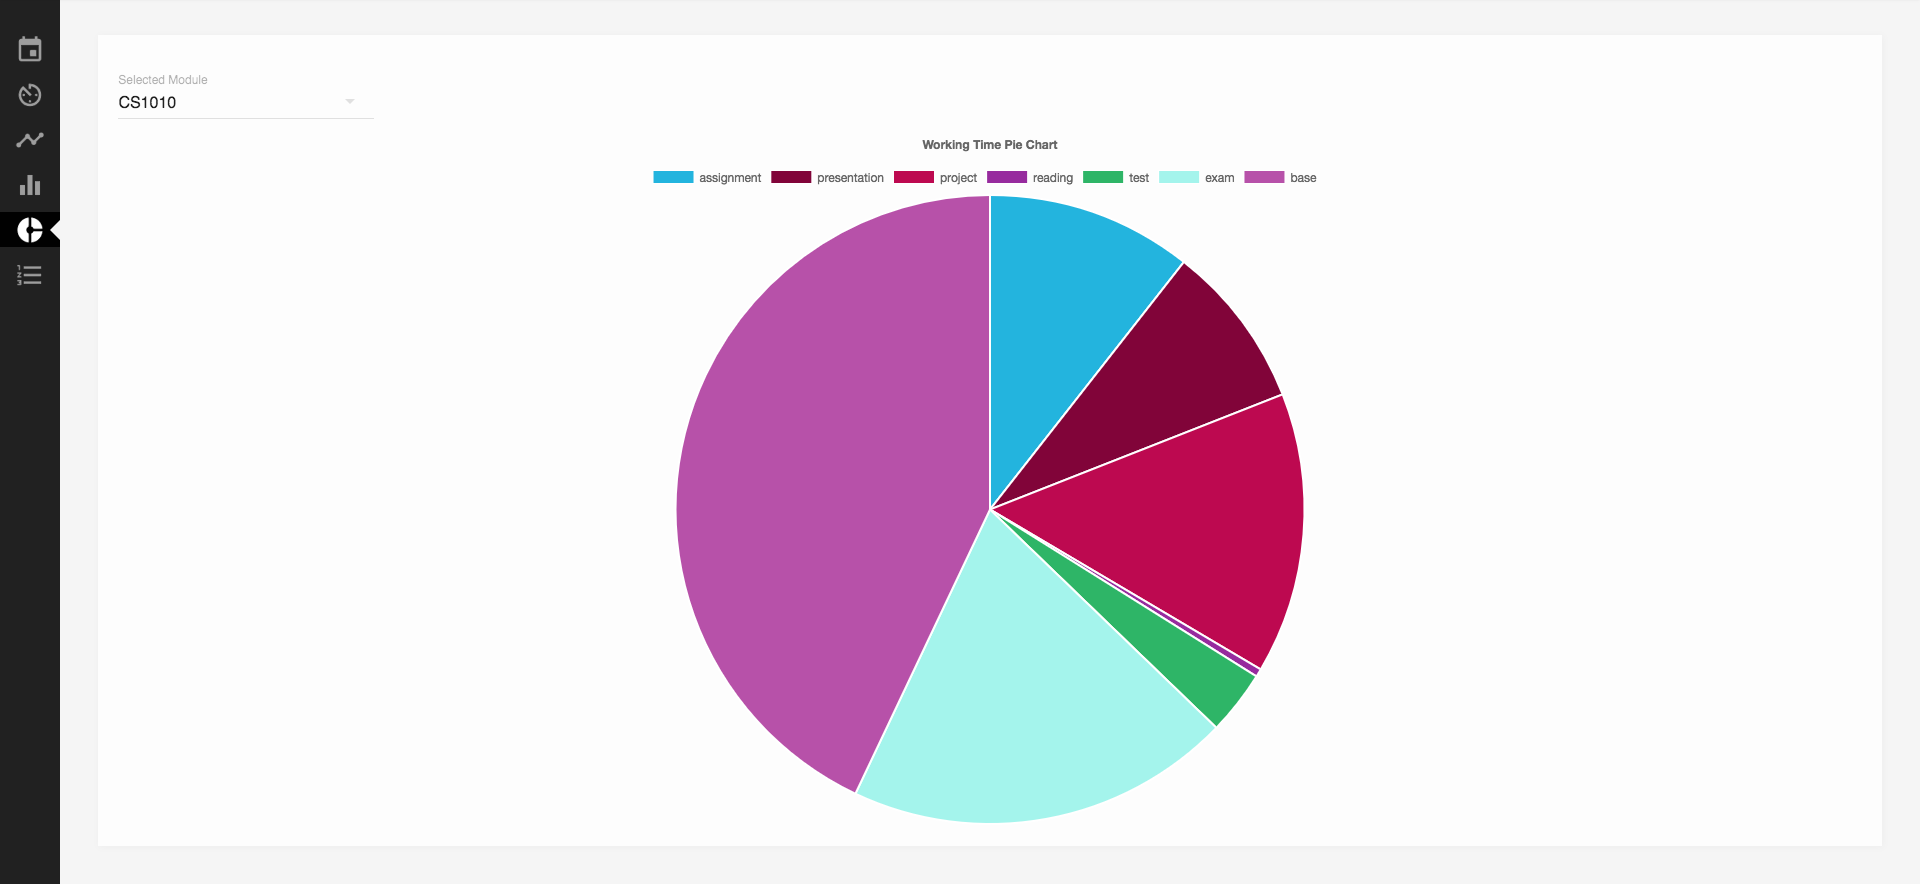
\includegraphics[width=\textwidth]{19}}
\caption{NUSWorks Screenshot (19)}
\label{screen-19}
\end{figure}

\begin{figure}
\frame{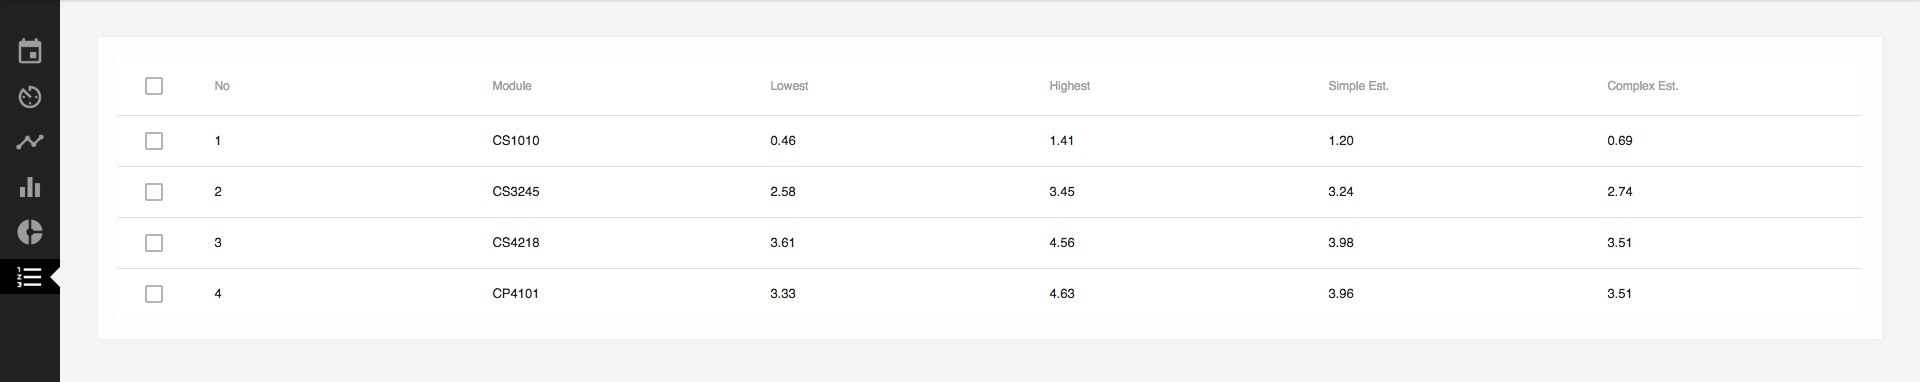
\includegraphics[width=\textwidth]{20}}
\caption{NUSWorks Screenshot (20)}
\label{screen-20}
\end{figure}

\chapter{External Libraries}
\begin{itemize}
	\item ReactJS: https://facebook.github.io/react/
	\item React Redux: https://github.com/reactjs/react-redux
	\item Webpack: https://webpack.github.io/
	\item Material UI: http://www.material-ui.com/\#/
	\item Sass: http://sass-lang.com/
	\item Yarn: https://yarnpkg.com/en/
	\item Flask: http://flask.pocoo.org/
	\item Python 3.6.1: https://www.python.org/downloads/release/python-361/
	\item MariaDB: https://mariadb.org/
	\item scikit-learn: http://scikit-learn.org/stable/
	\item Flask-SQLAlchemy: http://flask-sqlalchemy.pocoo.org/2.1/
	\item Flask-Marshmallow: https://flask-marshmallow.readthedocs.io/en/latest/
	\item Flask-Restful: https://flask-restful.readthedocs.io/en/0.3.5/
	\item Mocha: https://mochajs.org/
	\item Enzyme: http://airbnb.io/enzyme/
\end{itemize}

\end{document}
